V této kapitole jsou popsány metody použité v bakalářské práci. V
podkapitole~\ref{section:measurement} je rozebrán postup měření EKG záznamů a
použité zařízení. V kapitole~\ref{section:study} je charakterizována kontrolní
skupina probandů a sledované veličiny. V
kapitolách~\ref{section:offline_processing} a~\ref{section:online_processing} je
řešena metodologie online a offline zpracování a hodnocení EKG signálu.
Kapitola~\ref{section:statistical_methods} pojednává o statistickém zpracování
výsledků.

\subsection{Měření EKG signálů}
\label{section:measurement}
Pro účely zpracování a analýzy EKG signálu, které jsou náplní této bakalářské
práce, bylo provedeno pilotní měření krátkodobých záznamů srdeční aktivity na 5
probandech. Postup měření je specifikován v
kapitole~\ref{section:measurement_methodology}. Měřící zařízení je popsané v
následující kapitole.

\subsubsection{Měřící zařízení}
\label{section:measurement_device}
Zařízení použité k měření srdeční aktivity byl Holterův monitor (viz
Obr.~\ref{fig:device}), zajištěný vědeckým týmem Biomechaniky a asistivních
technologií. Skládá se ze dvou komponent: samotné zařízení a 3-svodový EKG kabel
s 3.5~\si\mm~jack konektorem. Vzorkovací frekvence zařízení je 500~\si\Hz.

Přenos dat ze zařízení probíhá bezdrátově na lokální sítí (WLAN), ke které je
třeba zařízení připojit pomocí volně dostupné mobilní aplikace \textit{ESPTouch:
SmartConfig}~\cite{ESPAPP} podle postupu níže. \textit{ESP-TOUCH} je protokol, umožňující
vestavěným systémům (embedded systémy) jednoduché připojení k Wi-Fi sítím pomocí
chytrých mobilních zařízení~\cite{esptouch}. K záznamu dat byla použita
aplikace, naprogramovaná v rámci této práce, jménem \textit{BBPM (Better bpm)},
která se zařízením komunikuje přes protokol \textit{Modbus}~\cite{modbus}.
Aplikace \textit{BBPM} je detailněji popsána v
kapitole~\ref{section:offline_processing}.

\begin{figure}[H]
    \begin{center}
        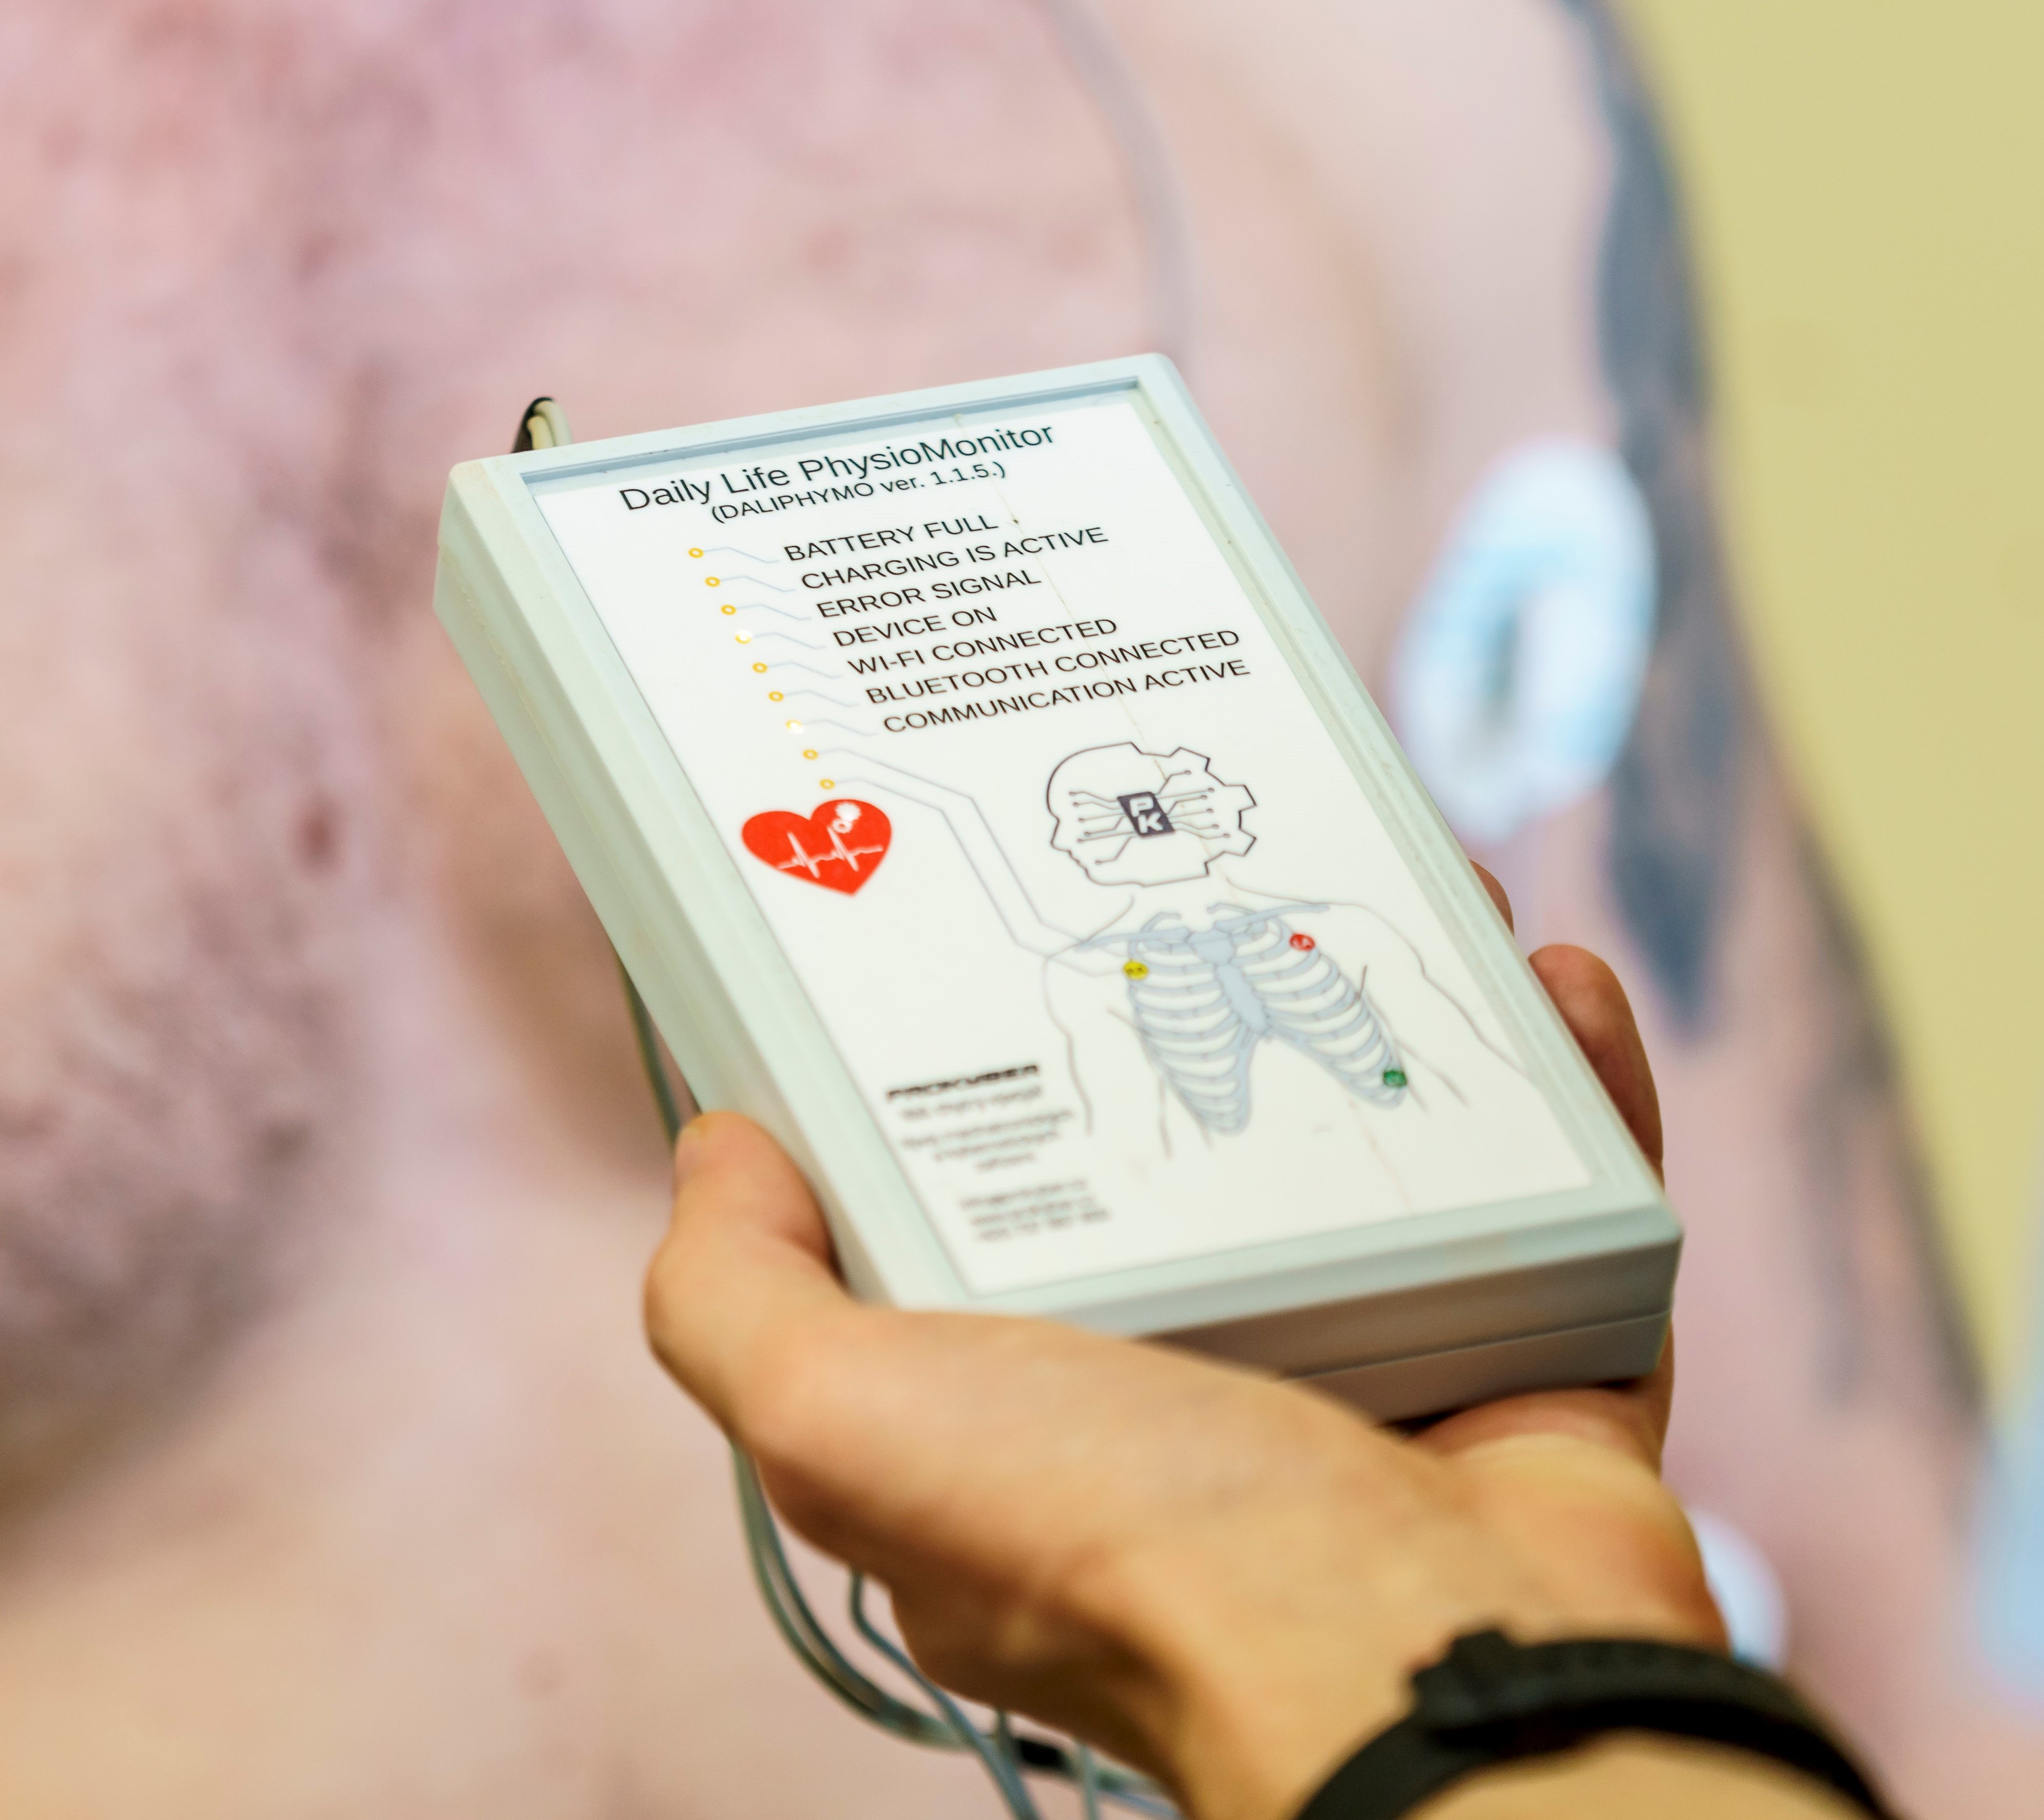
\includegraphics[width=0.9\textwidth]{device/holter1}
        \caption{Měřící zařízení s příslušenstvím}
        \label{fig:device}
    \end{center}
\end{figure}

Holterův monitor musí být při připojování k bezdrátové sítí v bezprostřední
blízkosti chytrého zařízení, kterým bude konfigurován. Postup pro připojení
měřícího zařízení k WLAN sítí je následující:
\begin{enumerate}
    \item Připojení chytrého mobilního zařízení, které bude sloužit ke
          konfiguraci Holterova monitoru, k požadované WLAN sítí, kde bude
          probíhat komunikace.
    \item Přepnutí měřícího zařízení do režimu konfigurace stiskem tlačítka
          \textbf{Config}, které se nachází na horní ploše okraje zařízení.
    \item Spuštění aplikace \textit{ESPTouch: SmartConfig}.
    \item Ověření správně vybrané WLAN sítě pomocí identifikátoru \textbf{SSID}
          v horní části úvodní obrazovky aplikace (Obr.~\ref{fig:app_screen1}).
    \item Vyplnění hesla v kolonce \textbf{Password} náležícího zvolené WLAN
          sítí. Ostatní parametry jsou ponechány ve výchozím stavu.
    \item Stisk tlačítka \textbf{Confirm} v dolní části aplikace pro zahájení
          konfigurace a připojení Holterova monitoru k vybrané sítí.
\end{enumerate}

Pokud se měřící zařízení připojilo úspěšně k vybrané WLAN sítí, objeví se
notifikace jako na Obr. \ref{fig:app_screen2} a zároveň je navázané spojení
indikované rozsvícenou LED kontrolkou na předním panelu Holterova monitoru u položky
\textbf{WI-FI CONNECTED}. Při nezdařeném pokusu připojení je nutné opakovat
kroky od bodu 2 nebo případně zkontrolovat stav baterie Holterova monitoru.

\begin{figure}[h]
    \centering
    \begin{subfigure}[b]{0.45\textwidth}
        \centering
        \textcolor{cyan}{\fboxrule=1.5pt\fboxsep=0pt\fbox{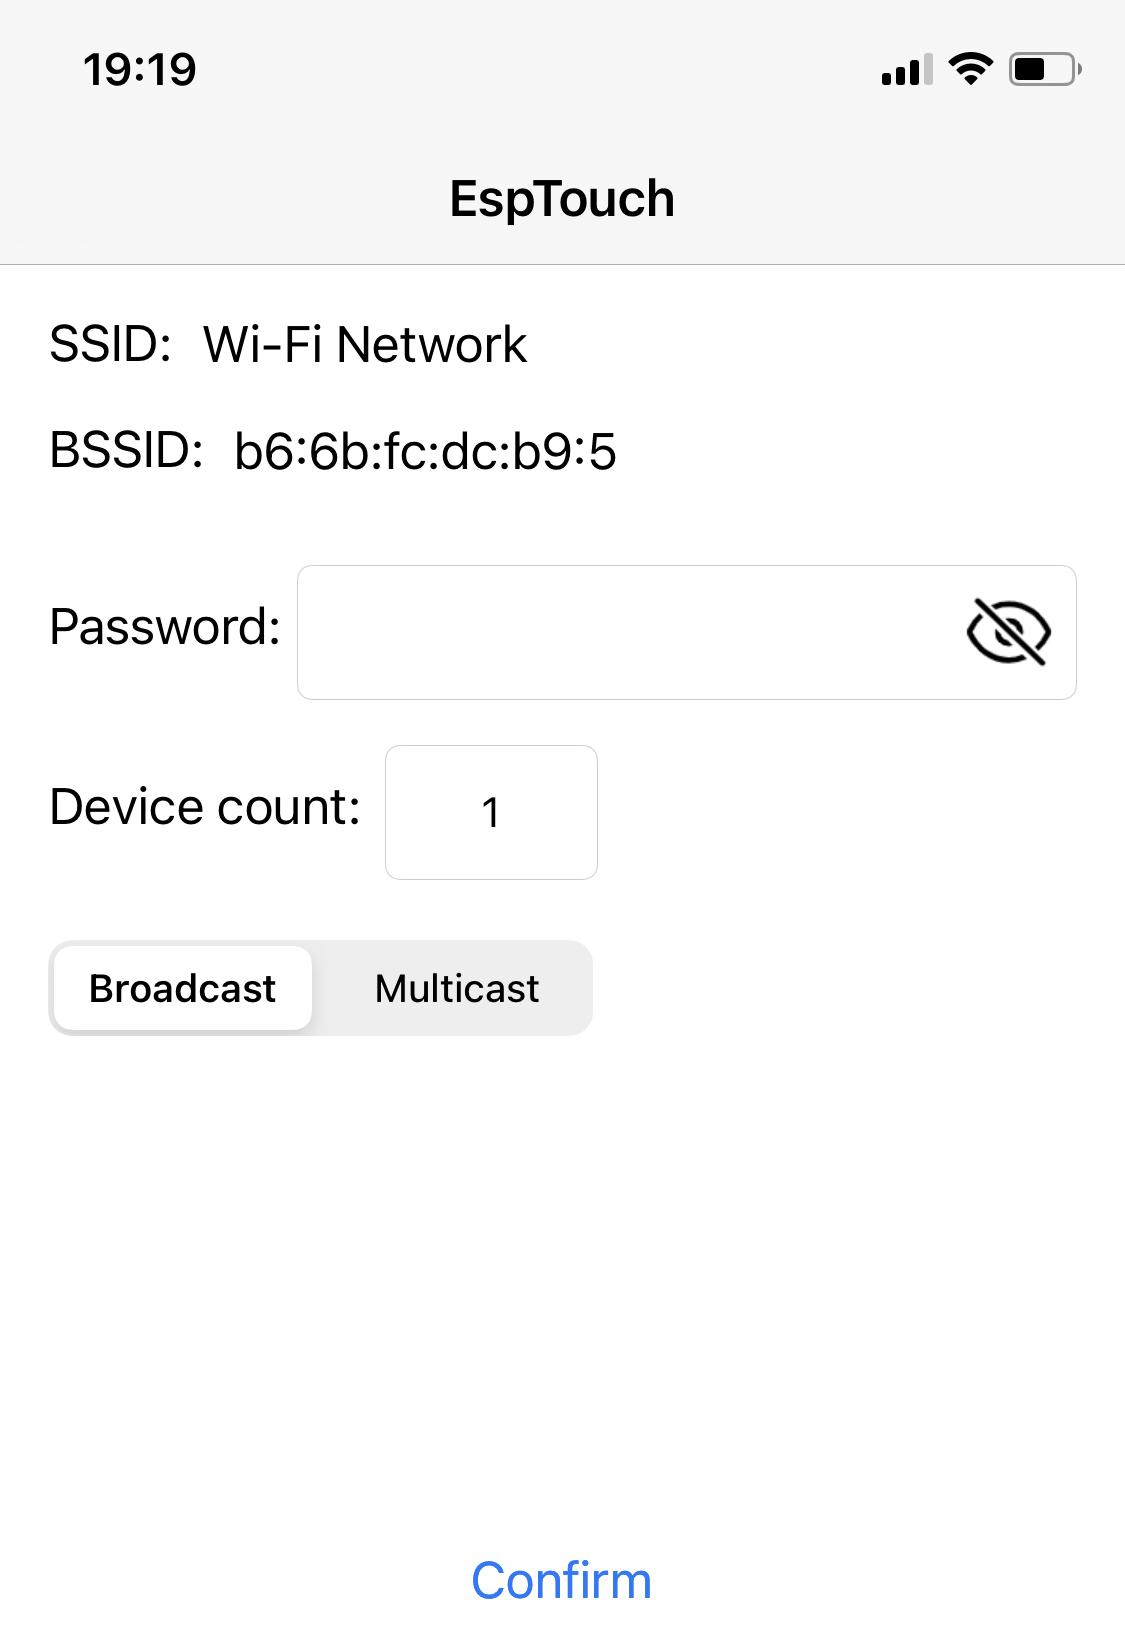
\includegraphics[width=0.8\linewidth]{device/app_screen1}}}
        \caption{Úvodní obrazovka aplikace}
        \label{fig:app_screen1}
    \end{subfigure}
    \hfill
    \begin{subfigure}[b]{0.45\textwidth}
        \centering
        \textcolor{cyan}{\fboxrule=1.5pt\fboxsep=0pt\fbox{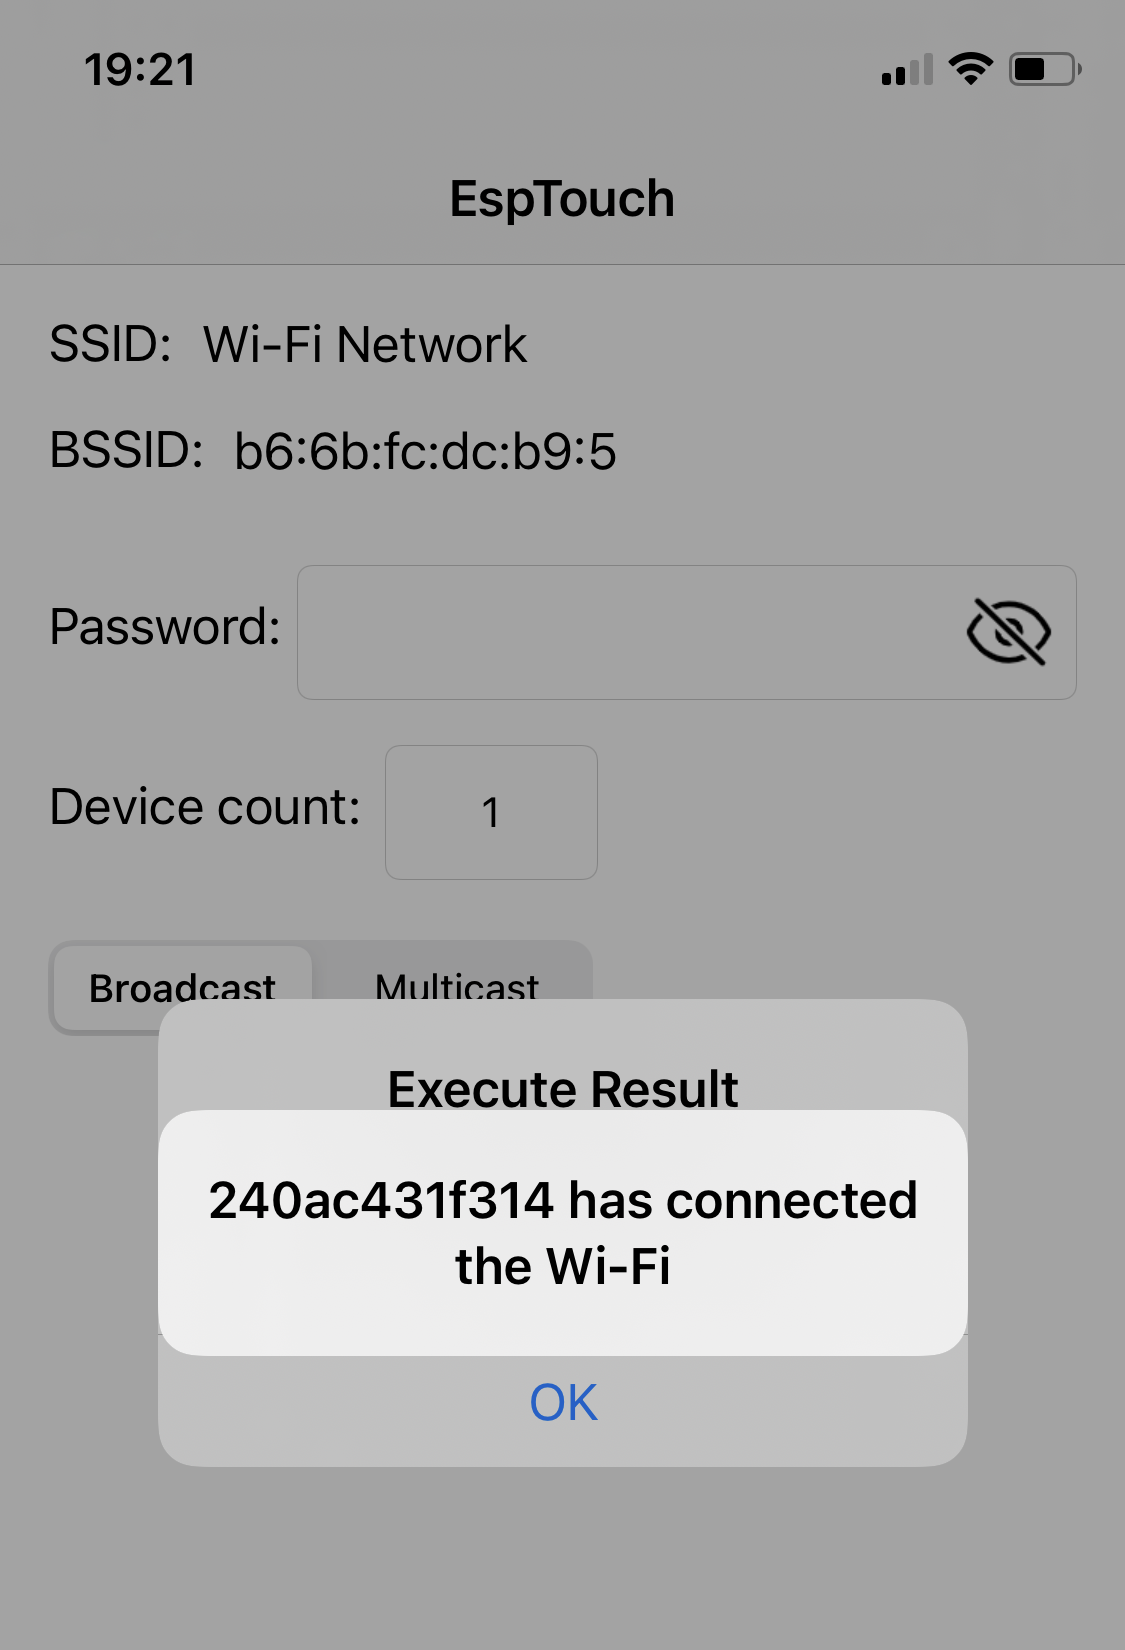
\includegraphics[width=0.8\linewidth]{device/app_screen2}}}
        \caption{Notifikace úspěšného připojení}
        \label{fig:app_screen2}
    \end{subfigure}
    \caption{Konfigurace měřícího zařízení v aplikaci \textit{ESPTouch:
            SmartConfig}~\cite{ESPAPP}}
    \label{fig:esptouch_app}
\end{figure}

\subsubsection{Metodika měření}
\label{section:measurement_methodology}
Metodika měření spočívá v krátkodobém záznamu srdeční aktivity ve dvou odlišných
situacích. Před měřením je na subjekt připojeno měřící zařízení, popsané v
sekci~\ref{section:measurement_device}, pomocí adhezivních EKG elektrod (viz
Obr.~\ref{fig:device_usage}). Jedná se o bipolární hrudní 3-svodové zapojení
elektrod (viz kapitola~\ref{section:electrocardiography}). Měření každého
záznamu trvá 10 minut, přičemž se jedná o dva 5 minutové spojité úseky. Subjekt
nesmí být před měřením vystaven fyzické ani psychické zátěži. Během měření v
prvním 5 minutovém úseku je subjekt po celou dobu v klidu. V druhém 5 minutovém
úseku je subjekt vystaven situaci stimulující kognitivní zátěž v podobě
Stroopova testu. Stroopův test je realizován formou videozáznamu a blíže je
popsán v následující kapitole. Postup měření je rozebrán v
sekci~\ref{section:measurement_process}.

\begin{figure}[h]
    \begin{center}
        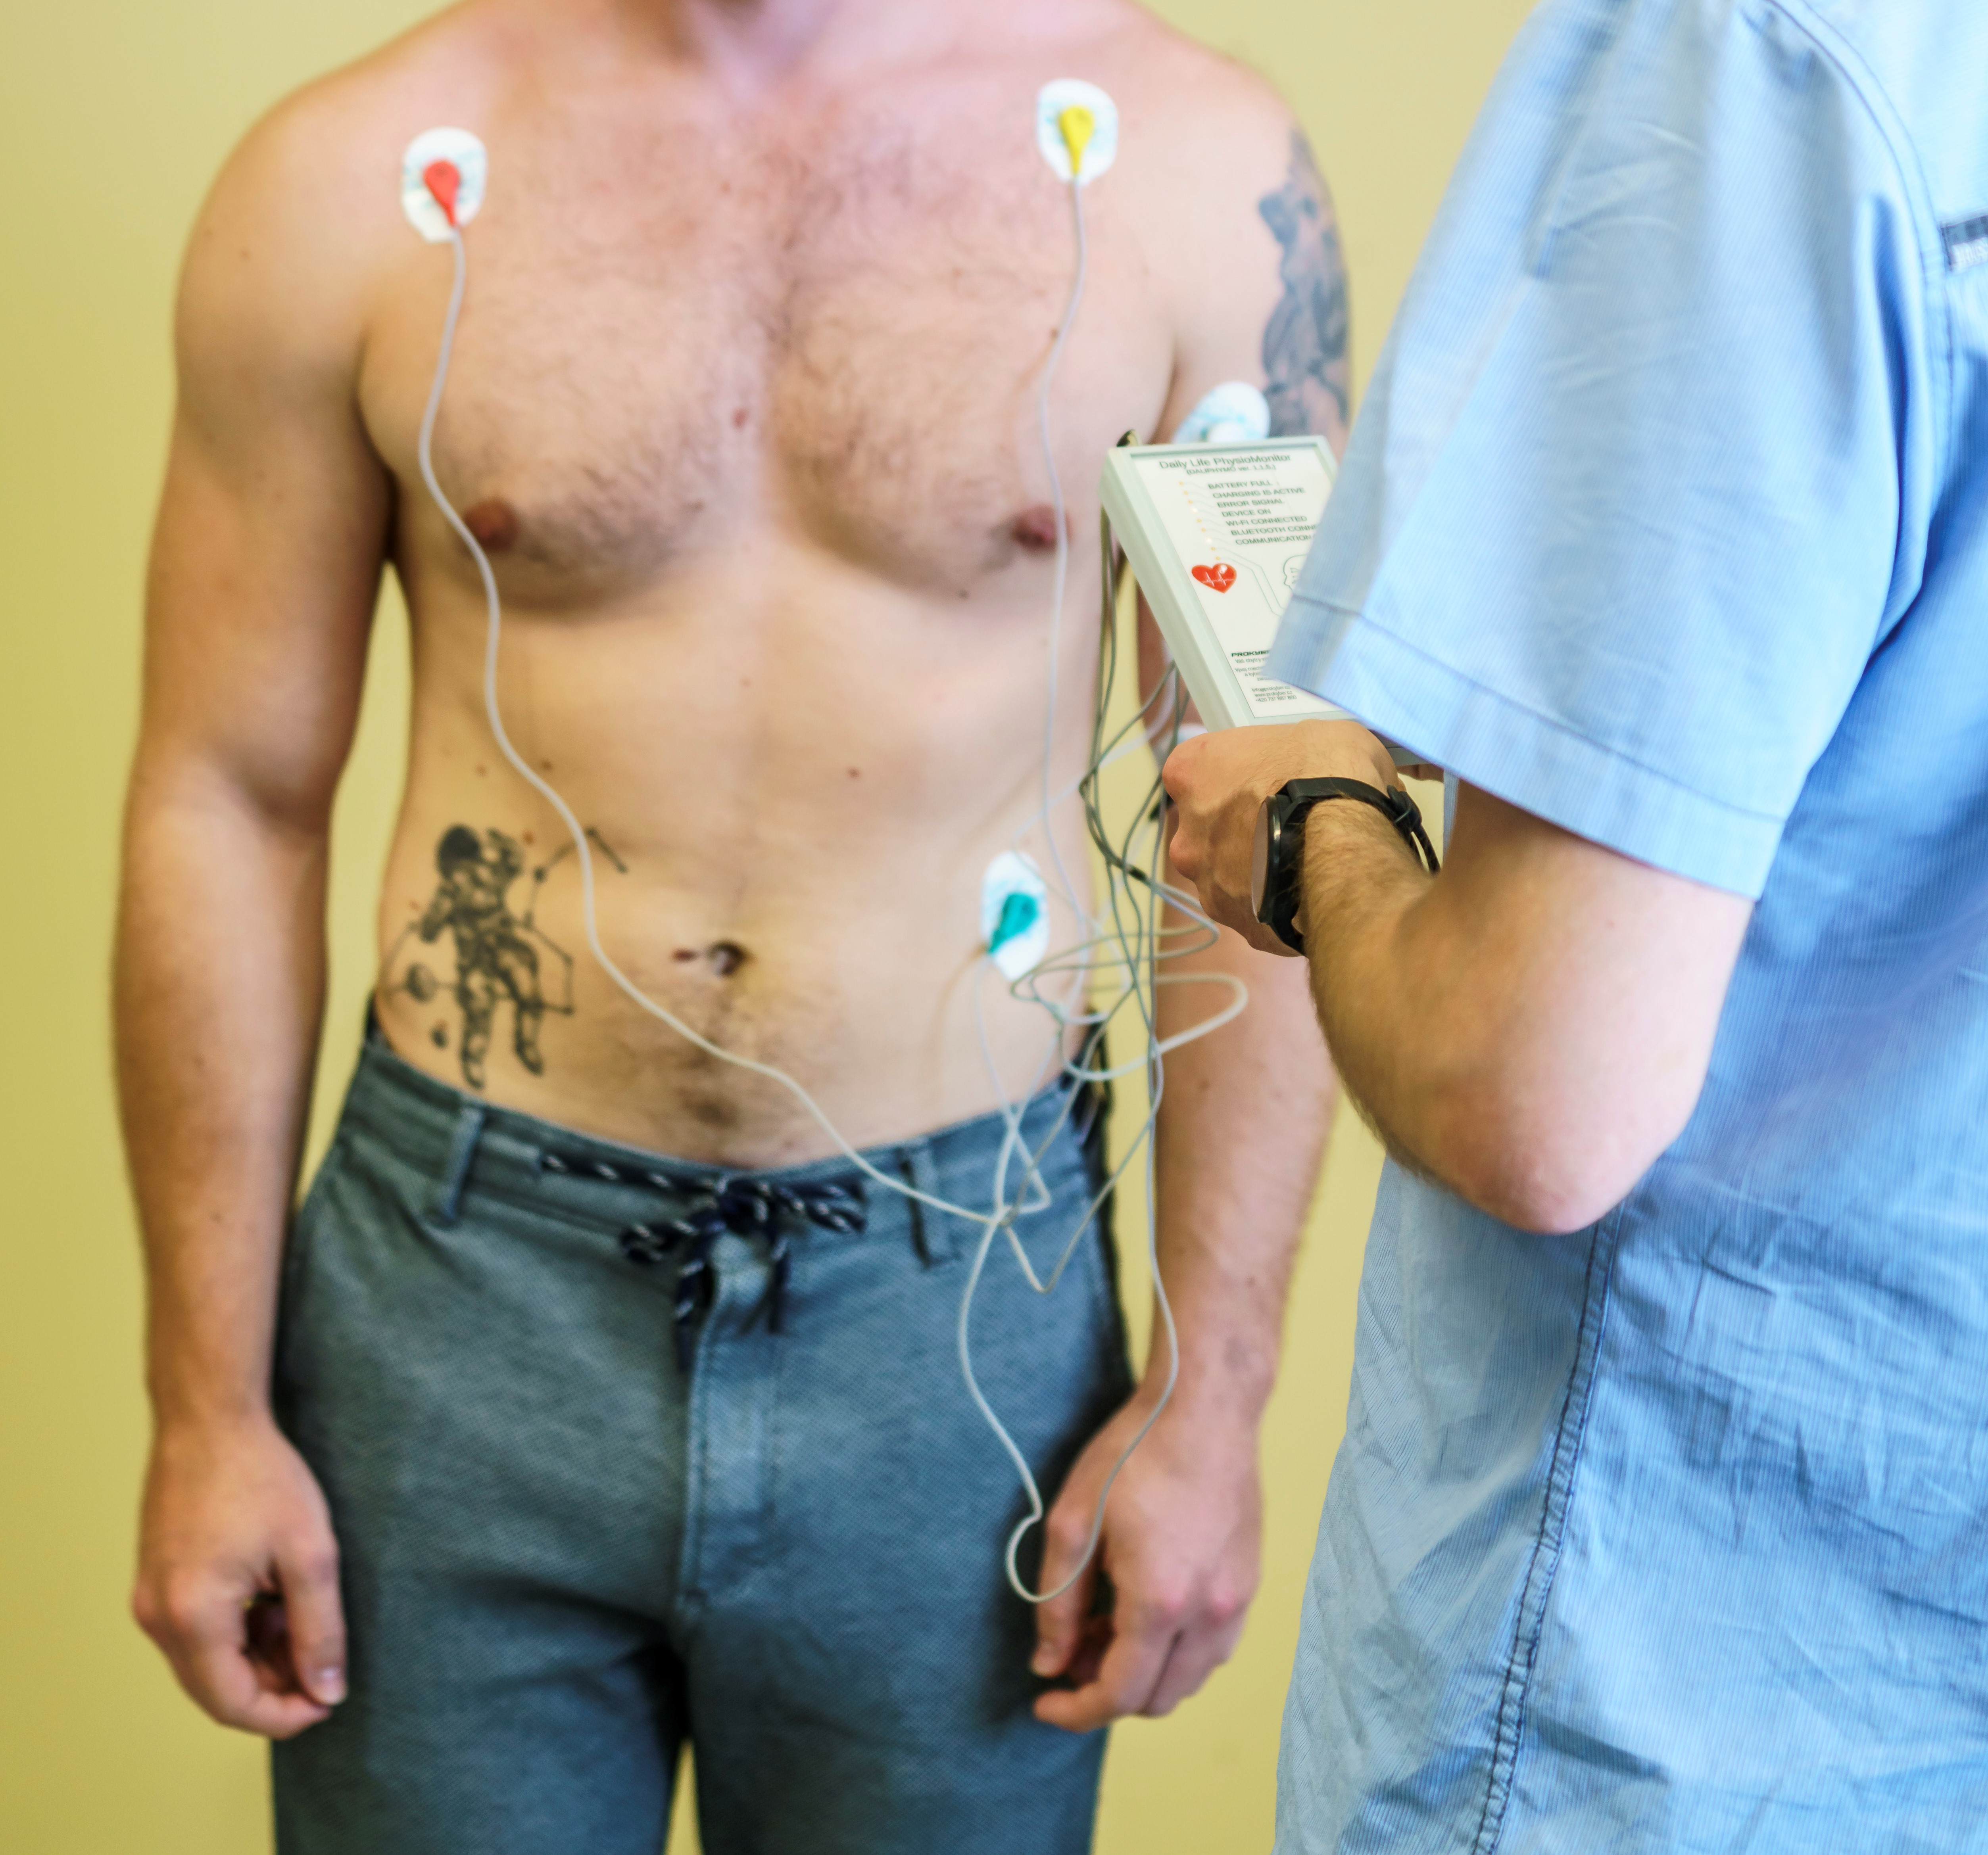
\includegraphics[width=0.7\textwidth]{device/holter2}
        \caption{Měření srdeční aktivity}
        \label{fig:device_usage}
    \end{center}
\end{figure}

\subsubsection{Stroopův test}
\label{section:stroop_test}
Stroopův test (viz Obr.~\ref{fig:stroop}) se řadí mezi psychologické testy osobnosti a byl primárně navržený
pro testování percepční zátěže. Postupem času se možnosti jeho využití
rozšiřovaly~\cite{Svoboda1999}. Dnes je Stroopův test jeden z nejběžnějších
neuropsychologických testů používaný k hodnocení  a stimulaci kognitivní
zátěže~\cite{Scarpina2017}.

\begin{figure}[h]
    \begin{center}
        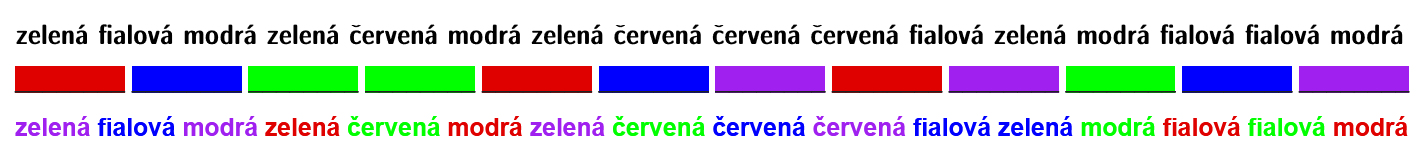
\includegraphics[width=1\textwidth]{figures/stroop}
        \caption{Příklad Stroopova testu~\cite{stroopWiki}}
        \label{fig:stroop}
    \end{center}
\end{figure}

Princip testu spočívá ve třech po sobě následujících krocích. Prvním krokem je
přečtení řady slov, která jsou napsána černou barvou a označují několik barev
(nejčastěji červená, žlutá, zelená a modrá). Dalším krokem je pojmenování každé
jednotlivé barvy v další řadě tvořené barevnými obdélníky. Posledním krokem je
přečtení řady slov, které jsou napsána barevně, ale význam slova této barvě
neodpovídá~\cite{Svoboda1999}.

\subsubsection{Postup měření}
\label{section:measurement_process}
Postup záznamu srdeční aktivity u jednotlivých probandů sestává z
následujících kroků:
\begin{enumerate}
    \item Konfigurace měřícího zařízení podle postupu v sekci~\ref{section:measurement_device}.
    \item Nalepení elektrod na měřeného probanda podle
          Obr.~\ref{fig:device_usage} a připojení příslušných EKG kabelů k elektrodám.
    \item Zapnutí aplikace \textit{BBPM}. Počítač na kterém běží aplikace musí
          být připojený ke stejné síti jako měřící zařízení.
    \item Nastavení aplikace stiskem tlačítka \textbf{Settings} a vyplněním IP
          adresy a portu měřícího zařízení do kolonek \textbf{Host} a \textbf{Port} v
          kartě \textbf{General}.
    \item Ověření validity spojení stiskem tlačítka \textbf{Test connection}.
    \item Připojení aplikace k měřícímu zařízení stiskem tlačítka
          \textbf{Apply} a následně \textbf{Ok}.
    \item Zahájení záznamu srdeční aktivity stiskem tlačítka \textbf{Record} a
          vybrání cílové destinace, kde bude soubor po ukončení záznamu uložen.
    \item Ukončení záznamu po 10 minutách opětovným stiskem tlačítka \textbf{Record}.
\end{enumerate}

\subsection{Studie}
\label{section:study}
Pilotní měření EKG záznamů bylo prováděno na lidských subjektech, tudíž je nutné
mít informovaný souhlas měřených probandů a souhlasné stanovisko etické komise.

\subsubsection{Stanovisko etické komise}
Sběr dat proběhl v rámci výzkumu \textit{Zpátky za volant -- Diagnostický a
rehabilitační nástroj pro osoby po poškození mozku}. Výzkum byl schválen etickou
komisí FBMI ČVUT. Stanovisko etické komise je uvedeno v Příloze
A (viz sekce~\ref{pdf:souhlas}) společně s informovaným souhlasem.

\subsubsection{Kontrolní skupina probandů}
\label{section:probands}
Za účelem otestovaní navrženého řešení (viz kapitola~\ref{section:thesis_aims}) byla naměřena a
zaznamenána srdeční aktivita podle postupu~\ref{section:measurement_process} u
kontrolní skupiny 5 probandů ve věkovém rozmezí 21--23 let bez diagnostikovaných
kardiovaskulárních onemocnění.

\subsubsection{Sledované statistické veličiny}
\label{section:selected_stats_vals}
Výstupem aplikace použité k záznamu srdeční aktivity (viz kapitola~\ref{section:online_processing}) jsou soubory formátu CSV,
kde každý řádek reprezentuje naměřenou výslednou amplitudu elektrické srdeční
aktivity v daný časový okamžik. Díky znalosti vzorkovací frekvence zařízení lze
snadno ke každému záznamu vypočítat časový vektor a pracovat tak v časové
oblasti.

V závislosti na studii byly vybrány následující sledované statistické parametry
Poincarého grafu s vyžitím metody konstrukce elipsy (viz
kapitola~\ref{section:hrv_methods}):
\begin{itemize}[noitemsep]
    \item \textbf{SD1}~\textit{(Standard Deviation)} -- směrodatná odchylka R-R
          intervalů hlavní osy elipsy,
    \item \textbf{SD2}~\textit{(Standard Deviation)} -- směrodatná odchylka R-R
          intervalů vedlejší osy elipsy,
    \item \textbf{SD1/SD2}~\textit{(Standard Deviation ratio)} -- poměr směrodatných odchylek SD1 a SD2.
\end{itemize}

\subsection{Offline zpracování EKG záznamu}
\label{section:offline_processing}
Zpracování EKG záznamů se orientuje podle diagramu na Obr.
\ref{fig:diagram_offline_processing} a je realizováno v prostředí 
\textit{MathWorks MATLAB 2021a}~\cite{MATLAB} s využitím \textit{Signal Processing
Toolboxu}~\cite{matlabSPT}. Jednotlivé části zpracování EKG záznamu jsou rozebrány v
následujících kapitolách.

\begin{figure}[H]
    \centering
    \begin{tikzpicture}[node distance=2.5cm, thick, scale=0.8, every node/.style={scale=0.8}]
        \node (start) [startstop, text width=2cm] {EKG záznam};
        \node (pro1) [process, right of=start, xshift=1.5cm] {Předzpracování};
        \node (pro2) [process, right of=pro1, xshift=1.5cm, text width=3cm] {Detekce komponentů};
        \node (pro3) [process, right of=pro2, xshift=1.5cm, text width=3cm] {Zpracování komponentů};
        \node (stop) [startstop, right of=pro3, xshift=1.5cm, text width=3cm] {Hodnocení záznamu};

        \draw [arrow] (start) -- (pro1);
        \draw [arrow] (pro1) -- (pro2);
        \draw [arrow] (pro2) -- (pro3);
        \draw [arrow] (pro3) -- (stop);
    \end{tikzpicture}
    \caption{Diagram offline zpracování EKG záznamu}
    \label{fig:diagram_offline_processing}
\end{figure}

\subsubsection{Předzpracování signálu}
\label{section:preprocessing}
Nezbytný krok pro jakoukoliv další práci s biosignálem je jeho filtrace. Před
navržením samotného filtru byl proveden rozbor EKG záznamů pomocí FFT. EKG
signál je tak převeden z časové domény do frekvenční funkcí
\texttt{fft(X)}~\cite{matlabFFT}. Z teorie je znám, v jakých frekvencích se
vyskytuje užitečný EKG signál nebo jeho komponenty a v jakých nežádoucí vlivy
(viz kapitola~\ref{section:ecg_processing_theory}). Tyto znalosti byly při
návrhu filtru a posuzování spektra EKG signálu využity. Pro zlepšení představy o
potenciálních artefaktech a užitečných frekvencích byla provedena FFT analýza i
na několika samotných PQRST segmentech. Na Obr.~\ref{fig:spectral_analysis} lze
vidět FFT analýzu EKG signálu a jednoho PQRST segmentu. Z examinace vizuální
stránky spektra plyne několik východisek pro tvorbu filtru. Jsou zde pohybové
artefakty společně s kolísáním nulové izolinie. Ve frekvenčním spektru a v
částech signálu se dále objevuje nepatrný širokopásmový šum, způsobený
myopotenciály. Ve frekvenčním spektru lze vidět tyto nežádoucí složky přibližně
mezi frekvencemi od 0 do 7,5~\si\Hz.

\begin{figure}[h]
    \begin{center}
        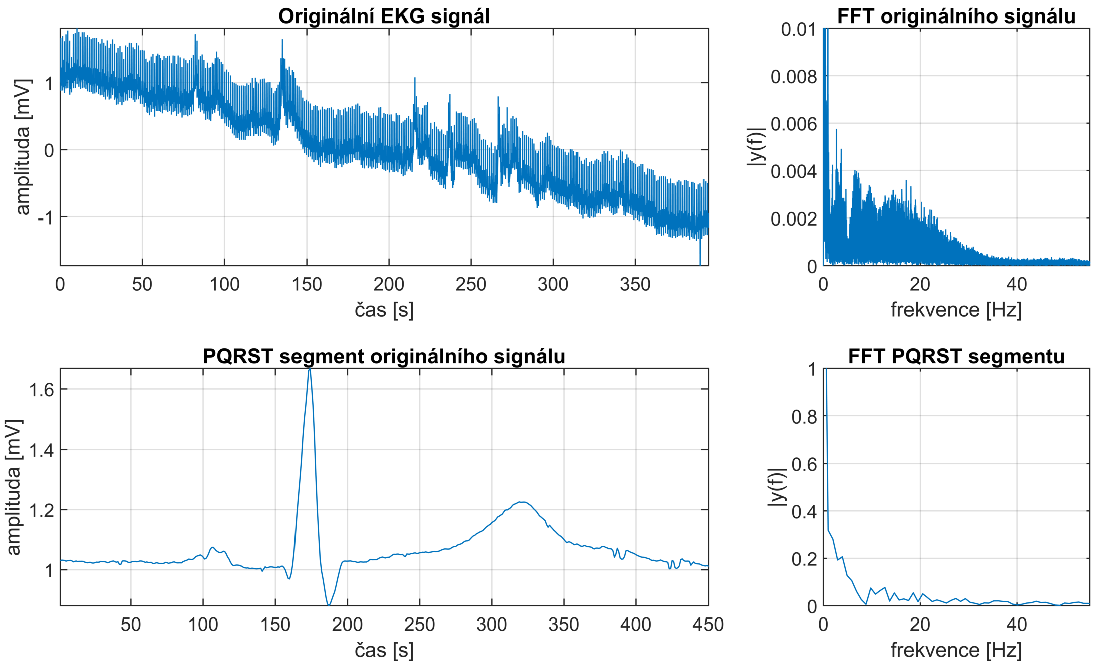
\includegraphics[width=1\textwidth]{figures/spectral_analysis}
        \caption{FFT analýza EKG signálu a QRS komplexu}
        \label{fig:spectral_analysis}
    \end{center}
\end{figure}

Po FFT analýze byl pro potlačení nežádoucích prvků použit pro každý EKG záznam
digitální filtr FIR (viz níže) typu pásmová propust s propustnými frekvencemi v rozmezí
7,5--35~\si\Hz. Filtr byl navržen metodou Kaiserova okna~\cite{Chavan2006},
které je definováno následovně~\cite{Oppenheim1999}:
\begin{equation}
    \label{eq:kaiser1}
    w[n] =
    \begin{cases}
        \frac{I_0[\beta\sqrt{(1-[(n-\alpha)/\alpha]^2)}]}{I_0(\beta)}, & 0 \leq n \leq M \\
        0,                                                           & \text{jinak}.
    \end{cases}
\end{equation}
kde $w$ označuje vypočítané koeficienty, $M$ je počet vzorků, $\alpha=M/2$ a
$I_0(\cdot)$ reprezentuje nultý řád modifikované Besselovy funkce prvního
druhu~\cite{BesselFcn}. Jelikož je potřeba dosáhnout specifického útlumu $A$
(viz kapitola~\ref{section:ecg_processing_theory}), definoval Kaiser parametr
$\beta$ k úpravě zvlnění propustného a závěrného pásma
následovně~\cite{Oppenheim1999}:
\begin{equation}
    \beta =
    \begin{cases}
        0,1102(A-8,7),                      & A > 50            \\
        0,5842(A-21)^{0,4} + 0.07886(A-21), & 21 \leq A \leq 50 \\
        0,                                  & A < 21.
    \end{cases}
\end{equation}

Filtr byl realizován funkcí \texttt{bandpass(x,fpass,fs)}~\cite{matlabBANDPASS}.
Druhou části předzpracování tvoří filtrace zvýrazňující QRS komplexy, konkrétně
R vlny. Použitá metoda pro zvýraznění vychází z vlastností derivace a vyšších
amplitud R vln. Filtrovaný signál je diferencován použitím pěti-bodové diference
prvního řádu dle následujícího vztahu:
\begin{equation}
    \label{eq:differentiation}
    y[n] = \frac{1}{8}(2x[n] + x[n-1] - x[n-3] - 2x[n-4])
\end{equation}
kde $n \geq 5$, $y[n]$ reprezentuje vzorek diferencovaného signálu a $x[n]$
hodnotu původního vzorku. Diference zároveň potlačuje vlivy P a T vln.
Dále je diferencovaný signál umocněn a QRS regiony jsou
následně jednotlivě sloučeny a zvýrazněny využitím zpětné
kumulace~\cite{Wang2017}:
\begin{equation}
    \label{eq:backward_cumulation}
    Bc(n) = \sum_{i=n}^{n+Ww-1} |y(i)|
\end{equation}
s pevnou délkou okna $Ww$ v rozsahu nejdelšího normálního trvání jednoho QRS
komplexu (0,12~\si\s)~\cite{Wang2017}. Ke kumulaci je využívána funkce
\texttt{cumsum(A)}~\cite{matlabCUMSUM}.

\begin{figure}[h!]
    \begin{center}
        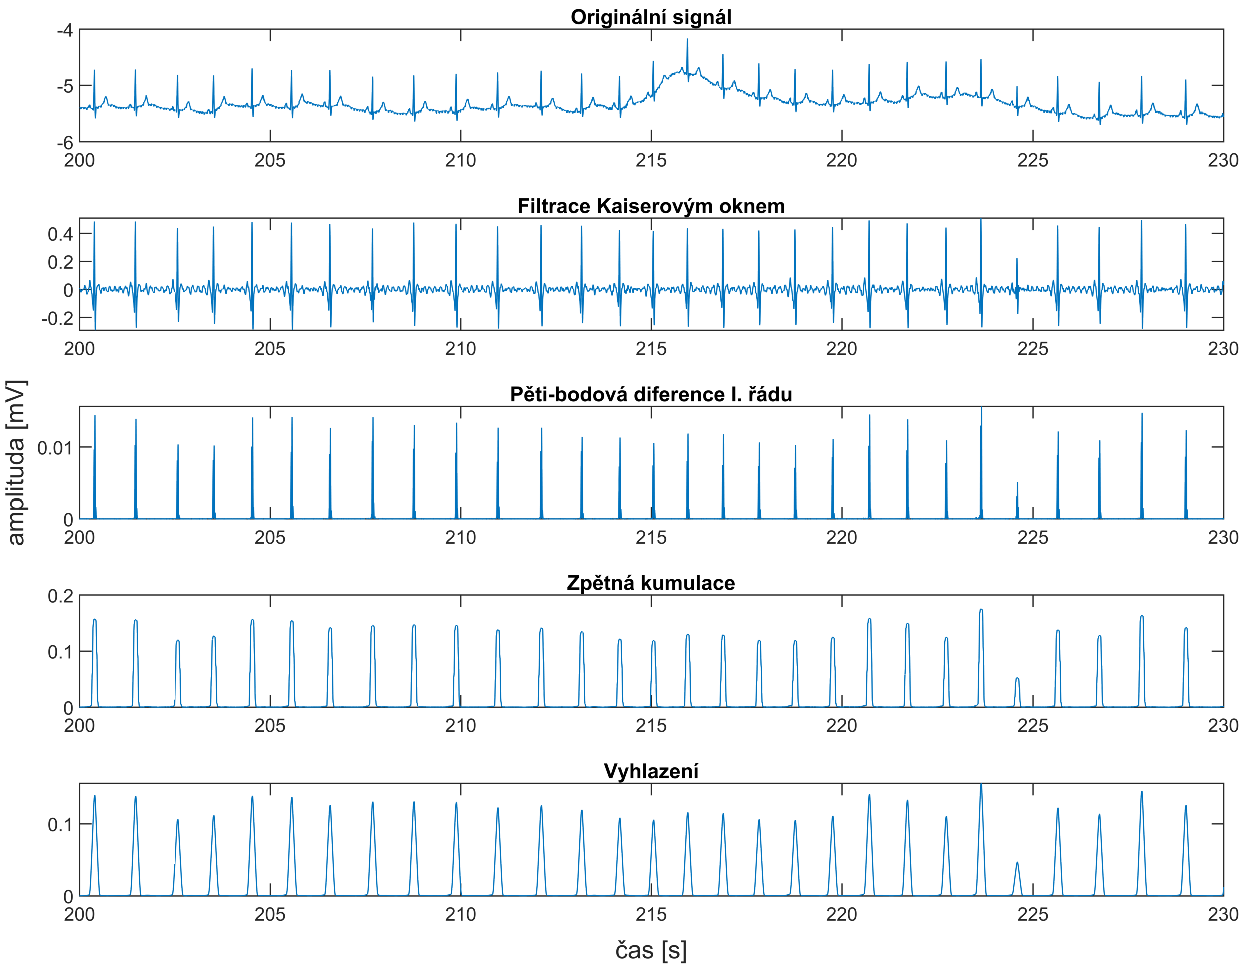
\includegraphics[width=1\textwidth]{figures/preprocessing_steps}
        \caption{Jednotlivé kroky předzpracování EKG signálu}
        \label{fig:preprocessing_steps}
    \end{center}
\end{figure}

Poslední krok předzpracování je vyhlazení vzniklých vrcholů konvolucí použitím
funkce \texttt{conv(u,v)}~\cite{matlabCONV}. Principiálně se jedná o vyhlazení 
plovoucím průměrem s délkou okna 60 vzorků. Délka 60 vzorků je
stejně jako u zpětné kumulace doba trvání QRS komplexu, převedena z času na
počet vzorků pomocí vzorkovací frekvence (500~\si\Hz). Vizuálně lze vidět
jednotlivé kroky předzpracování signálu na Obr.~\ref{fig:preprocessing_steps}.

\subsubsection{Detekce komponentů}
\label{section:components_detection}
Detekce komponentů tvoří nezbytnou část, od které se odvíjí hodnocení EKG
záznamu. Cílem detekce je spolehlivě identifikovat a lokalizovat specifické
komponenty, nejčastěji QRS komplexy, které jsou předmětem analýzy EKG záznamu.
Díky detekovaným komponentům lze signál využitím detekovaných veličin
segmentovat a hodnotit. V první řadě se nejčastěji volí detekce R vln na základě
jejich vysoké amplitudy.

Za účelem detekce R vln byl implementován a modifikován algoritmus
podle~\cite{Nabian2018}, inspirovaný Pan-Tompkinsovou metodou QRS
detekce~\cite{Pan1985} (viz kapitola~\ref{section:components_detection_theory}).
Algoritmus vychází z následujících kroků:
\begin{enumerate}
    \item Iterativní hledání globálních maximálních amplitud s použitím
          plovoucího okna $W$ o délce 400~\si\ms~(0,4~\si\s):
          \begin{gather}
              R_{max} = max(W_i^{L,R}) \nonumber \\
              L = R = \frac{0.4~Fs}{2}, \quad L,R \in \mathbb{Z^+} \nonumber \\
              W_i^{L,R} = \{x_{i-L},...,x_i,...,x_{i+R}\}, \quad \forall i \in \{1+L,...,N-R\}
          \end{gather}
          kde $N$ je počet detekovaných R vln, $Fs$ vzorkovací frekvence, $R_i$
          potenciální R vlna, $x_i$ střed okna a $L$ spolu s $R$ posun od středu
          plovoucího okna. Nalezená maxima nacházející se uprostřed plovoucího
          okna jsou označeny jako potenciální R vlny.
    \item Eliminace všech R vln nižších než než prahová hodnota $Th_{Amp}$, která je v
          každé iteraci rovna 75 \% z průměru amplitud posledních 8 detekovaných
          R vln. Iniciálně je prahová hodnota $Th_{Amp}$ nastavena jako:
          \begin{gather}
              n = 2~Fs, \quad n \in \mathbb{Z^+} \nonumber \\
              Th_{Amp} = \frac{1}{3} max(\{x_1,x_2,x_3,...,x_n\})
          \end{gather}
    \item Výpočet R-R intervalů ($RR_i$) diferencí detekovaných R vln ($R_i$):
          \begin{equation}
              RR_i = R_{i} - R_{i-1}, \quad \forall i \in \{2,...,N\}
          \end{equation}
          Následně je provedena iterativní kontrola vypočítaných R-R intervalů.
          Intervaly delší než prahová hodnota $Th_{RR}$ indikují chybějící R
          vlnu, která je doplněna jako maximální amplituda v rozmezí délky
          plovoucího okna následovně:
          \begin{gather}
              n = \frac{0.4~Fs}{2}, \quad n \in \mathbb{Z^+} \nonumber \\
              R_m = max(\{R_{i+n},...,R_i,...,R_{i+1-n}\}), \quad \forall i \in \{1,...,N\}
          \end{gather}
          kde $R_m$ je doplněná R vlna. Prahová hodnota $Th_{RR}$ je počátečně
          nastavena jako:
          \begin{equation}
              Th_{RR} = 1.66~RR_1
          \end{equation}
\end{enumerate}

Délka plovoucího okna se řídí fyziologickým limitem hodnoty srdečního rytmu v
případech, jako jsou například supraventrikulární tachykardie (SVT) nebo flutter
síní, kde dosahuje srdeční frekvence přibližně 300 úderů za minutu (5 úderů za
sekundu)~\cite{Haberl2012,Goldberger2017}. Dva sousední QRS komplexy se tedy
nemůžou vyskytnout blíže než 200~\si\ms.

\begin{figure}[h]
    \begin{center}
        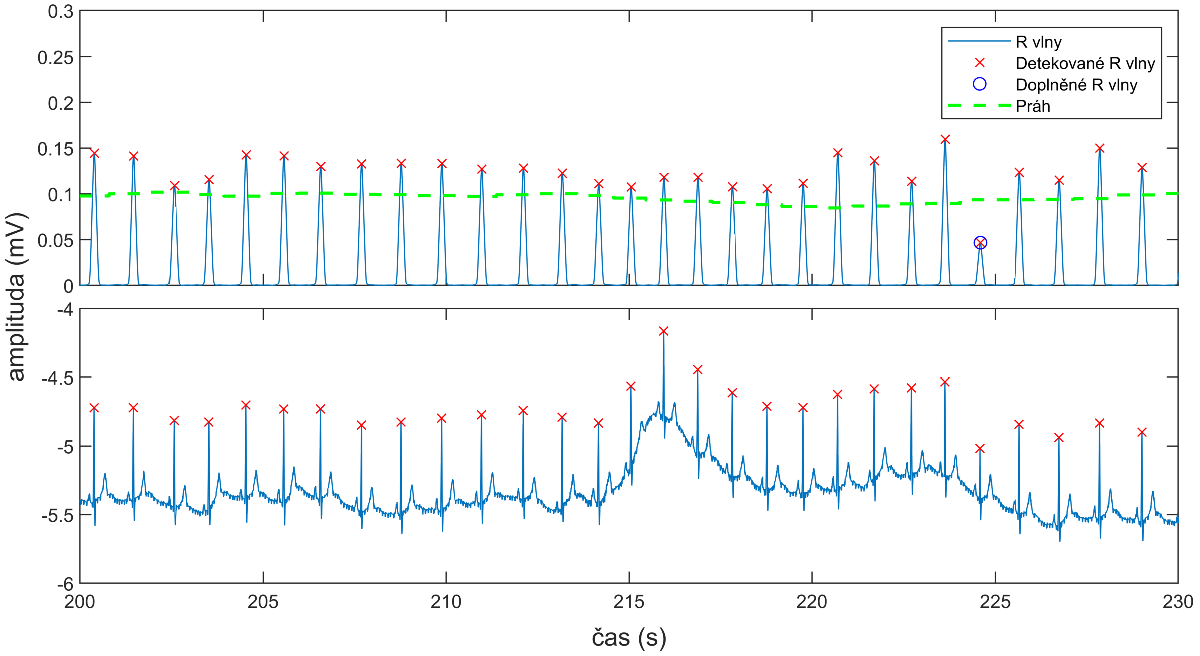
\includegraphics[width=1\textwidth]{figures/detection}
        \caption{Vizualizace detekovaných R vln}
        \label{fig:detection}
    \end{center}
\end{figure}

Na Obr.~\ref{fig:detection} lze vidět zeleně vyznačený
adaptivní práh, který se mění podle 2. kroku výše a doplněnou R vlnu, která
nebyla detekovaná v 1. kroku ale až ve 3. a následně doplněna.

\begin{figure}[H]
    \begin{center}
        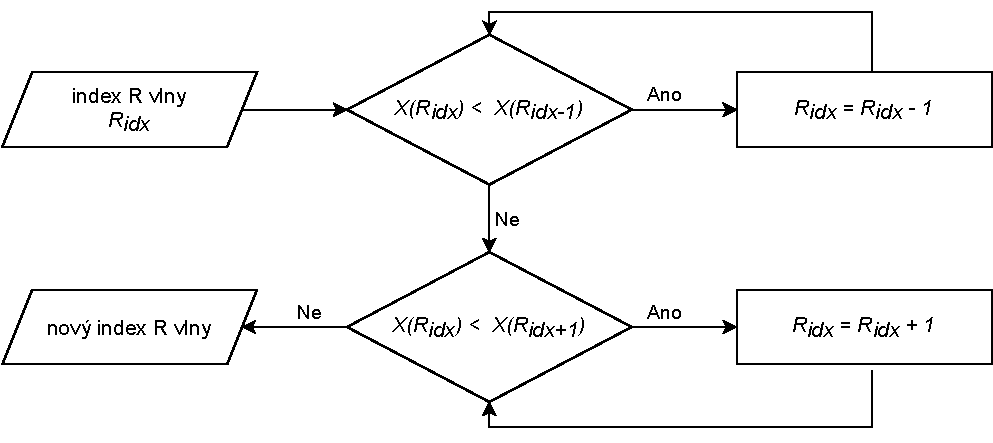
\includegraphics[width=0.87\textwidth]{diagrams/fixpeaks}
        \caption{Algoritmus relokalizace detekovaných R vln}
        \label{fig:fixpeaks}
    \end{center}
\end{figure}

Pro zobrazení detekovaných vln v původním signálu (viz. Obr.~\ref{fig:detection})
byla zavedena metoda relokalizace, která upraví pozice
detekovaných R vln tak, aby souhlasily v původním EKG záznamu. Díky tomu lze
vizuálně ověřit spolehlivost algoritmu nebo evaluovat detekci v oblastech s očekávaným
výskytem artefaktů, které jsou více zatížené nežádoucími vlivy. Postup metody se řídí
diagramem na Obr.~\ref{fig:fixpeaks}, kde $X$ reprezentuje množinu hodnot EKG
signálu.

\subsubsection{Zpracování detekovaných komponentů}
\label{section:components_processing}
V případě analýzy variability srdečního rytmu (viz kapitola~\ref{section:hrv})
je nutné tuto veličinu vypočítat z detekovaných komponentů. Diferencí mezi
sousedícími R vlnami v čase jsou vypočítány R-R intervaly neboli časová
variabilita mezi jednotlivými údery srdce. Stejně jako EKG záznam, tak i R-R
intervaly jsou zatížené artefakty a mohou představovat abnormální hodnoty.
Zdrojem artefaktů jsou nejčastěji falešně nebo nesprávně detekované či chybějící
R vlny a ektopický rytmus, který společně s invalidně detekovanými R vlny
vytváří sekvence dlouhých a krátkých srdečních period. Vizuálně lze artefakty
identifikovat, jako velké náhlé změny či kolísání v grafu jako je tomu na
Obr.~\ref{fig:hrv_artifacts}. Podmínkou HRV analýzy je tedy použití N-N
intervalů (normal-to-normal), které představují korigované R-R intervaly.
Korekcí je myšleno potlačení nežádoucích artefaktů.

\begin{figure}[h]
    \begin{center}
        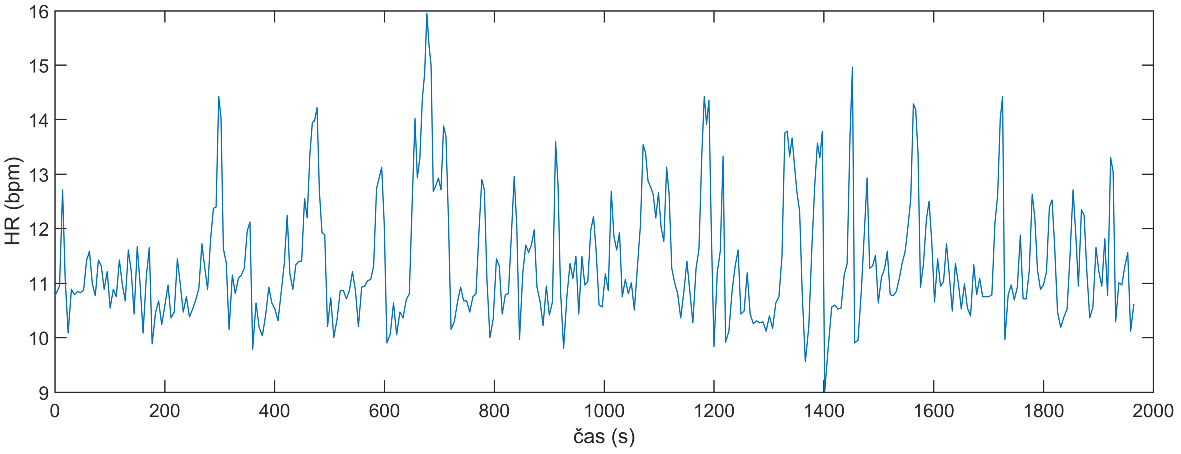
\includegraphics[width=1\textwidth]{figures/hrv_artifacts}
        \caption{HRV signál zatížený artefakty}
        \label{fig:hrv_artifacts}
    \end{center}
\end{figure}

K zajištění spolehlivé HRV analýzy a minimalizaci chyb byla implementována
automatická metoda pro detekci a korekci artefaktů HRV
podle~\cite{Lipponen2019}. Metoda je založená na adaptivním prahování s využitím
dvou pohyblivých prahových hodnot. V prvním kroku je vypočtena časová diference
všech detekovaných R-R intervalů $dRRs$, která slouží k rozlišení ektopických a
nesprávně detekovaných R vln od normálního sinusového rytmu~\cite{Lipponen2019}:
\begin{gather}
    dRRs_1 = 0 \nonumber \\
    dRRs_j = RR_j - RR_{j-1}, \quad \forall j \in \{2,...,N\}
\end{gather}
kde $N$ je počet R-R intervalů. Pro detekci abnormálních intervalů je nastaven
první práh $Th1$, který se adaptuje statistickým odhadem z časově proměnného
rozdělení $dRRs$ hodnot. Práh představuje sérii hodnot, definovaných produktem
faktoru $\alpha$ a mezikvartilového rozpětí $QD$ 91 okolních $dRRs$ intervalů
následovně~\cite{Lipponen2019}:
\begin{equation}
    Th1 = \alpha~QD(|\{dRRs_{j-45},...,dRRs_{j+45}\}|), \quad \forall j \in \{46,...,N-45\}
\end{equation}
kde $\alpha$ je bezrozměrný škálovací faktor, jehož hodnota byla empiricky zvolena
5,2. Časová série $dRRs$ je následně normalizována prahovými
hodnotami~\cite{Lipponen2019}:
\begin{equation}
    dRR_j = \frac{dRRs_j}{Th1_j}, \quad \forall j \in \{1,...,N\}
\end{equation}

Veličiny $dRR$ jsou použité pro detekci ektopických, krátkých, dlouhých nebo
jednotlivě chybějících srdečních period porovnáním $|dRR|>1$. Pro zbylé případy
falešně pozitivní detekce R vln nebo jiných chyb, které nelze detekovat použitím
$dRR$, je definována série $mRRs$ jako rozdíl jednotlivých R-R intervalů a
mediánu 11 okolních hodnot~\cite{Lipponen2019}:
\begin{equation}
    mRRs_j = RR_j - median(\{RR_{j-5},...,RR_{j+5}\}), \quad \forall j \in \{6,...,N-5\}
\end{equation}

Vzhledem k tomu, že při srdeční frekvenci 60 bpm se v rámci falešně pozitivní detekce 
srdečního cyklu hodnota $mRRs$ pohybuje okolo -0,5~\si\s, a při detekci
vynechaného cyklu se blíží k 1~\si\s, nelze použít jednotný práh. Aby bylo
možné použít stejný práh pro všechny případy identifikace artefaktu jako v
předešlé sérii $dRRs$, jsou hodnoty $mRRs$ upravené následující
podmínkou~\cite{Lipponen2019}:
\begin{equation}
    mRRs_j =
    \begin{cases}
        2~mRRs_j, & \forall mRRs_j < 0    \\
        mRRs_j,   & \forall mRRs_j \geq 0
    \end{cases}
    , \quad \forall j \in \{1,...,N\}
\end{equation}

Při stejné srdeční frekvenci (60 bpm) se hodnoty $mRRs$ po úpravě blíží k
0~\si\s~u normálního sinusového rytmu, 1~\si\s~ u vynechaných cyklů a k
--1~\si\s~ u nadbytečně detekovaných srdečních period. Stejně jako pro předchozí
sérii $dRRs$, tak i pro $mRRs$ je zaveden totožně definovaný práh
$Th2$~\cite{Lipponen2019}:
\begin{equation}
    Th2 = \alpha~QD(|\{mRRs_{j-45},...,dRRs_{j+45}\}|), \quad \forall j \in \{46,...,N-45\}
\end{equation}
a hodnoty $mRRs$ jsou následně normalizovány~\cite{Lipponen2019}:
\begin{equation}
    mRR_j = \frac{mRRs_j}{Th2_j}, \quad \forall j \in \{1,...,N\}
\end{equation}

Prahové hodnoty $Th1$ a $Th2$ vycházejí z předpokladu, že časová řada R-R
intervalů pochází z normálního rozdělení, který ve většině případech není
splněn, a proto dochází k chybným identifikacím artefaktů. K zamezení těchto
chyb je metoda doplněna klasifikačním rozhodovacím Algoritmem~\ref{algo:rr_decision}.

\begin{figure}[ht]
    \centering
    \begin{minipage}{.9\linewidth}
        \begin{algorithm}[H]
            \SetKw{Continue}{continue}
            \KwVstup{$S11$, $S12$, $dRR$, $mRR$, $medRR$, $RR$, $Th2$, $rr\_len$ -- Počet R-R}
            \KwVystup{List detekovaných artefaktů}
            List $\leftarrow$ \{\}\;
            \LinesNumbered
            \For{ $i \in \{1,\ldots,rr\_len-2\}$ }{
                $eq_1 \leftarrow (S11_i > 1) \land (S12_i < (-c_1 \times S11_i - c_1))$\;
                $eq_2 \leftarrow (S11_i < -1) \land (S12_i > (-c_1 \times S11_i + c_2))$\;
                $eq_3 \leftarrow sgn(dRR_i) \times dRR_{i+1} < -1$\;
                $eq_4 \leftarrow sgn(dRR_i) \times dRR_{i+2} < -2$\;
                $eq_5 \leftarrow |RR_i/2 - medRR_i| < Th2_i$\;
                $eq_6 \leftarrow |RR_i + RR_{i+1} - medRR_i| < Th2_i$\;
        
                \If{$|dRR_i| > 1$}{
                        \uIf{ $ eq_1 \land eq_2 $ }{
                            List.append('Ectopic beat'); \Continue;
                        }
                        \uElseIf{$|mRR_i| > 3 \land eq_3 \land eq_4$}{
                            \lIf{$eq_5$}{List.append('Missed beat'); \Continue}
                            \lElseIf{$eq_6$}{List.append('Extra beat'); \Continue}
                            \lElse{List.append('Long/short beat'); \Continue}
                        }
                        \Else{
                            List.append('Normal beat'); \Continue;
                        }
                    }
                }
            \caption{Detekce a klasifikace artefaktů}
            \label{algo:rr_decision}
        \end{algorithm}
    \end{minipage}
\end{figure}

Veličiny $c_1$ a $c_2$ jsou empiricky nastavené konstanty
podle~\cite{Lipponen2019}. Hodnoty $S11$ a $S12$ jsou definované v následujícím
odstavci.

Ektopický rytmus se v sérii hodnot $dRR$ projevuje jako sekvence záporné, kladné
a záporné hodnoty (NPN, N--Negative, P--Positive) nebo kladné, záporné a
kladné (PNP). Pomocí těchto vzorů je rozlišen ektopický rytmus od vynechaných
či nadbytečných srdečních cyklů nebo náhlých změn srdeční frekvence. 
Pro účely vizuálního hodnocení detekce ektopických
srdečních stahů je vytvořen dvoudimenzionální prostor $S1$
následovně~\cite{Lipponen2019}:
\begin{gather}
    S11_j = dRR_j, \quad \forall j \in \{1,...,N\} \nonumber \\
    S12_j =
    \begin{cases}
        max(\{dRR_{j-1}, dRR_{j+1}\}), & dRR_j > 0 \\
        min(\{dRR_{j-1}, dRR_{j+1}\}), & dRR_j < 0
    \end{cases}
    , \quad \forall j \in \{2,...,N-1\}
    \label{eq:subspace1}
\end{gather}
ve kterém se hodnoty $S11$ a $-S12$ zvětšují v rámci determinace NPN vzorem a
zmenšují u PNP případů. Na Obr.~\ref{fig:rr_process} lze vidět vizualizované
prostory $S1$ a $S2$ s vyznačenými hranicemi, vymezující detekované artefakty
podle~\eqref{eq:subspace1} a~\eqref{eq:subspace2}.

\begin{figure}[h]
    \begin{center}
        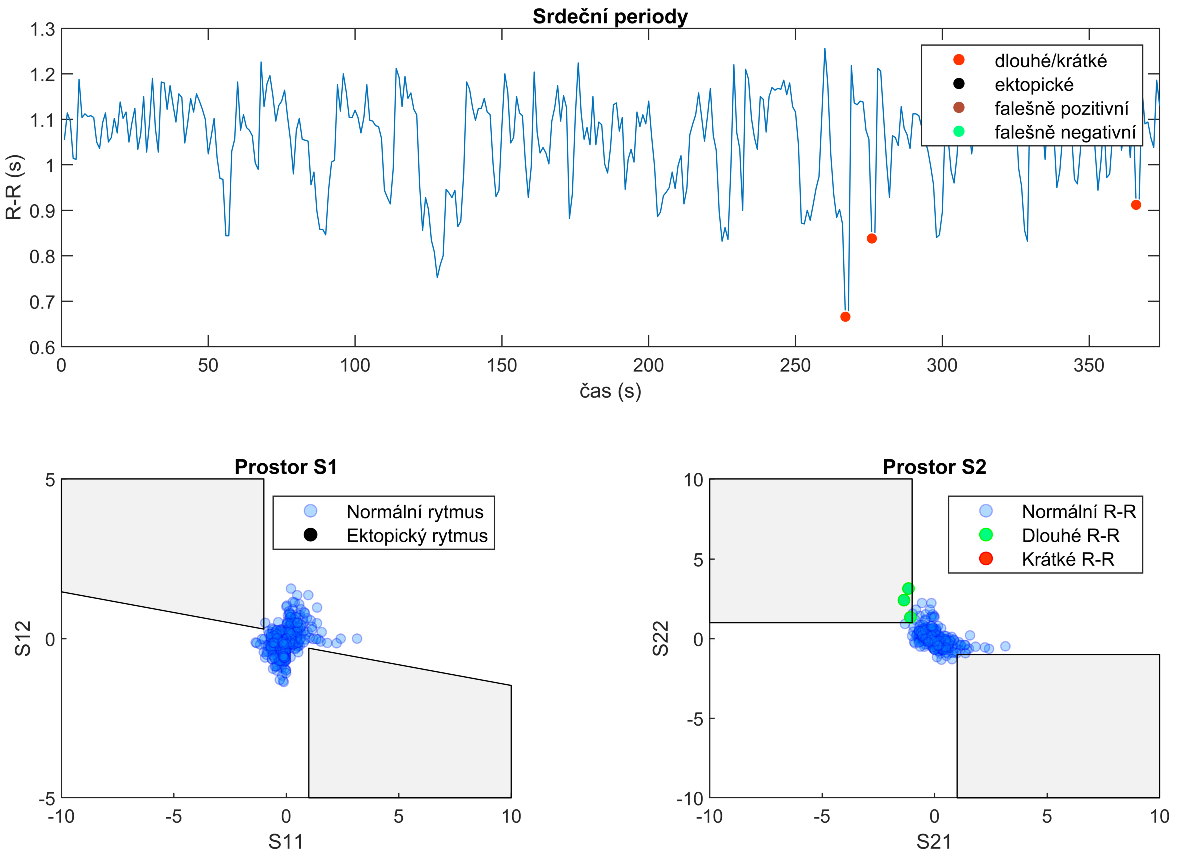
\includegraphics[width=1\textwidth]{figures/rr_process}
        \caption{Vizualizace detekovaných artefaktů}
        \label{fig:rr_process}
    \end{center}
\end{figure}

Dlouhé srdeční cykly včetně případů nedetekovaných R vln se projevují v $dRR$
sérií sekvencí PN, pomalými cykly NP a nadbytečnými periodami jako NNP nebo NPP. K
zobrazení těchto artefaktů a jejich detekčních hranic slouží 2D prostor $S2$
definovaný~\cite{Lipponen2019}:
\begin{gather}
    S21_j = dRR_j, \quad \forall j \in \{1,...,N\} \nonumber \\
    S22_j =
    \begin{cases}
        min(\{dRR_{j-1}, dRR_{j+1}\}), & dRR_j \geq 0 \\
        max(\{dRR_{j-1}, dRR_{j+1}\}), & dRR_j < 0
    \end{cases}
    , \quad \forall j \in \{2,...,N-1\}
    \label{eq:subspace2}
\end{gather}

Posledním krokem je korekce detekovaných artefaktů, která se řídí jejich typem a
přepočet nové série korigovaných R-R intervalů. Úprava je realizována
pro každý typ artefaktu následujícím způsobem~\cite{Lipponen2019}:
\begin{itemize}
    \item \textbf{Falešně pozitivní srdeční periody} -- odstranění
          nadbytečných, nesprávně detekovaných R vln, které jsou začátkem falešné
          periody.
    \item \textbf{Vynechané srdeční periody} -- přidání nových R vln, které
          rovnoměrně rozdělí korespondující R-R interval.
    \item \textbf{Dlouhé a krátké srdeční periody} -- interpolace a přidání
          nových R-R intervalů.
    \item \textbf{Ektopický rytmus} -- nahrazení ektopických period interpolovanými R-R intervaly.
\end{itemize}

\subsubsection{Analýza zpracovaného záznamu}
\label{section:analysis}
Pro analýzu EKG záznamů, konkrétně hodnocení HRV, byla zvolena nelineární
geometrická metoda Poincarého grafu s konstrukcí elipsy (viz
kapitola~\ref{section:hrv_methods}). Jedná se o bodový graf, kde každý bod tvoří
R-R interval vynesený proti následujícímu R-R intervalu. Prvním krokem k
sestrojení grafu je vytvoření časových vektorů následovně~\cite{Mazhar2007}:
\begin{gather}
    \overrightarrow{RR_i} = \{RR_1, RR_2,...,RR_{N}\} \\
    \overrightarrow{RR_{i+1}} = \{RR_2, RR_3,...,RR_{N-1}\}
\end{gather}
kde $N$ je celkový počet R-R intervalů. Dalším krokem je výpočet kvantitativních
parametrů Poincarého grafu SD1 a SD2, které zároveň slouží ke konstrukci
elipsy. Směrodatné odchylky SD1 a SD2 jsou vypočteny jako~\cite{Mazhar2007}:
\begin{equation}
    \text{SD1} = \sqrt{var(x1)}
    \quad \textrm{a} \quad
    \text{SD2} = \sqrt{var(x2)}
\end{equation}
kde $x_1$ a $x_2$ neboli hlavní a vedlejší osy elipsy jsou
rovny~\cite{Mazhar2007}:
\begin{equation}
    x_1 = \frac{\overrightarrow{RR_i}-\overrightarrow{RR_{i+1}}}{\sqrt{2}}
    \quad \textrm{a} \quad
    x_2 = \frac{\overrightarrow{RR_i}-\overrightarrow{RR_{i+1}}}{\sqrt{2}}
\end{equation}

\noindent Elipsa je konstruována využitím jejího vyjádření parametrickými
rovnicemi:
\begin{gather}
    \label{eq:ellipse_parametric}
    x = a \cos \theta \nonumber \\
    y = b \sin \theta
\end{gather}
kde $\theta \in \langle 0, 2\pi \rangle$, $a$ je šířka elipsy a $b$ je její
výška. Za výšku elipsy je dosazena hodnota SD1 a za šířku SD2. Hlavní osa
elipsy leží v případě Poincarého grafu na přímce dané předpisem $y=x$ a elipsa
je tak natočena o 45\degree~($\frac{\pi}{4}$). Vypočítané body z parametrického
vyjádření elipsy~(\ref{eq:ellipse_parametric}) je tedy nutné
rotovat následovně:
\begin{equation}
    \begin{bmatrix}
        X \\
        Y
    \end{bmatrix}
    =
    \overline{RR} +
    \begin{bmatrix}
        \cos \frac{\pi}{4} & -\sin \frac{\pi}{4} \\
        \sin \frac{\pi}{4} & \cos \frac{\pi}{4}
    \end{bmatrix}
    \cdot
    \begin{bmatrix}
        x \\
        y
    \end{bmatrix}
\end{equation}
kde $X$ a $Y$ jsou výsledné body po rotaci o 45\degree. $\overline{RR}$ je
vypočítaný průměr z R-R intervalů a je středem elipsy, do kterého je třeba
elipsu posunout přičtením této hodnoty k oběma souřadnicím. Proměnné $x$ a $y$
jsou předešle vypočítané souřadnice podle~\ref{eq:ellipse_parametric}. 
Realizované Poincarého grafy lze vidět v Příloze C (Obr.~\ref{fig:attachment_poincares_plots}).

\subsection{Online zpracování EKG záznamu}
\label{section:online_processing}
Pro zpracování EKG signálu v reálném čase bylo naprogramované multiplatformní
řešení s grafickým učitelským rozhraním (GUI) pojmenované \textit{BBPM -- Better
bpm}. Zpracování signálu se řídí stejným diagramem jako v
kapitole~\ref{section:offline_processing} na
Obr.~\ref{fig:diagram_offline_processing}. Motivací pro vznik aplikace je
spolupráce s Mgr. et Mgr. Ivetou Fajnerovou, Ph.D. z Národního ústavu duševního
zdraví (NÚDZ). Aplikace je využívána pro hodnocení duševního stavu osob ve
virtuální realitě. Detailněji je program popsán v následujících kapitolách.

\subsubsection{Aplikace pro hodnocení a sběr dat}
Program byl vytvořen pomocí skriptovacího jazyka
Python~\cite{python} s využitím frameworku \textit{PySide2} (viz
sekce~\ref{section:pyside}). Hlavním účelem programu je online zpracování a
vizualizace dat z měřicího zařízení, aby bylo možné sledovat a hodnotit
srdeční aktivitu měřené osoby v reálném čase. Aplikací lze data i
zaznamenávat a vzápětí uložit ve formátu CSV. K zajištěni minimální latence mezi
vizualizací zpracovaných dat a přijatými aktuálními daty, probíhá zpracování
signálu, jeho analýza a záznam paralelně (tzv. multithreading).

\subsubsection{Struktura aplikace}
Aplikaci lze rozdělit na dvě základní rozhraní, frontend a backend. Frontend
poskytuje interaktivní GUI společně s vizualizací zpracovaných dat (viz
kapitoly~\ref{section:gui}~a~\ref{section:visual}). V backend části probíhá v
jednotlivých vláknech (threadech) akvizice a záznam dat včetně výpočetních
procesů spojených se zpracováním EKG signálu (sekce~\ref{section:online_data_process}). 
Strukturu aplikace lze vidět na Obr.~\ref{fig:app_structure}.

\begin{figure}[h]
    \begin{center}
        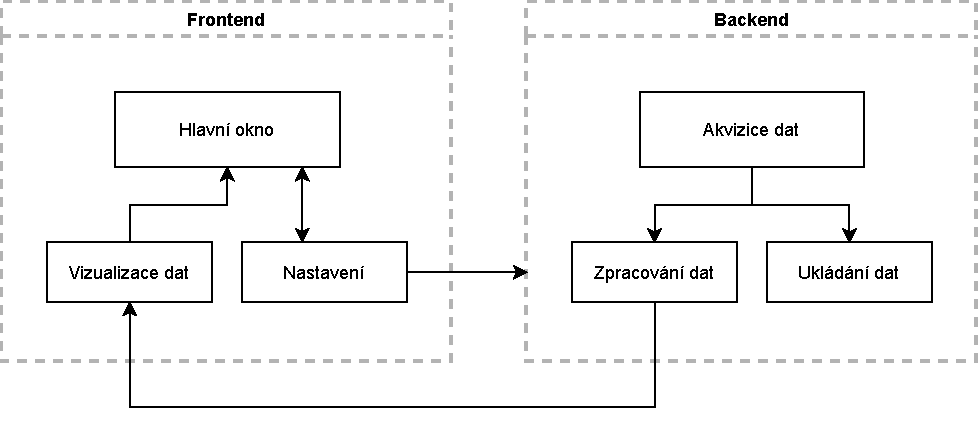
\includegraphics[width=0.9\textwidth]{diagrams/app_structure}
        \caption{Struktura aplikace \textit{BBPM}}
        \label{fig:app_structure}
    \end{center}
\end{figure}

\subsubsection{PySide framework}
\label{section:pyside}
\textit{PySide} představuje vazbu (binding) skriptovacího jazyka Python
na sadu GUI nástrojů populární knihovny \textit{Qt} \cite{Qt}. Díky tomu je
možné využívat aplikační rozhraní (API) knihovny \textit{Qt} v prostředí
Python. \textit{Qt} není pouze knihovna, ale celý nativní
multiplatformní framework pro vytváření softwaru s GUI, implementovaný v programovacím
jazyce \textit{C++}. V aplikaci \textit{BBPM} byla použita knihovna
\textit{PySide2}, která představuje port pro \textit{Qt5}.

\subsubsection{Uživatelské rozhraní}
\label{section:gui}
Grafické uživatelské rozhraní zajišťuje jednoduchou komunikaci mezi aplikací a
uživatelem pomocí interaktivních komponentů. Pro návrh a tvorbu GUI byl použit
nástroj \textit{Qt~Designer}~\cite{QtDesigner}, který je součástí knihovny
\textit{PySide2} a lze vidět na Obr.~\ref{fig:qt_designer}. Nástroj funguje na
principu \textit{WYSIWYG} editorů a umožňuje tak rychlou a intuitivní tvorbu
uživatelského rozhraní. V prostředí nástroje je vidět živý náhled aplikace v
podobě uživatelského okna~(\ref{fig:qt_designer}--\textbf{3}), které je hlavním
komponentem. Do hlavního okna lze z panelu č.~\textbf{1} přesouvat interaktivní
uživatelské prvky. Jednotlivé parametry prvků společně s hlavním oknem (např.
výška a šířka) lze upravovat v panelu č.~\textbf{2}. Vytvořené GUI je možné
následně exportovat v podobě Python kódu nebo formátu UI kompatibilním s knihovnou 
\textit{PySide}.

\begin{figure}[h]
    \begin{center}
        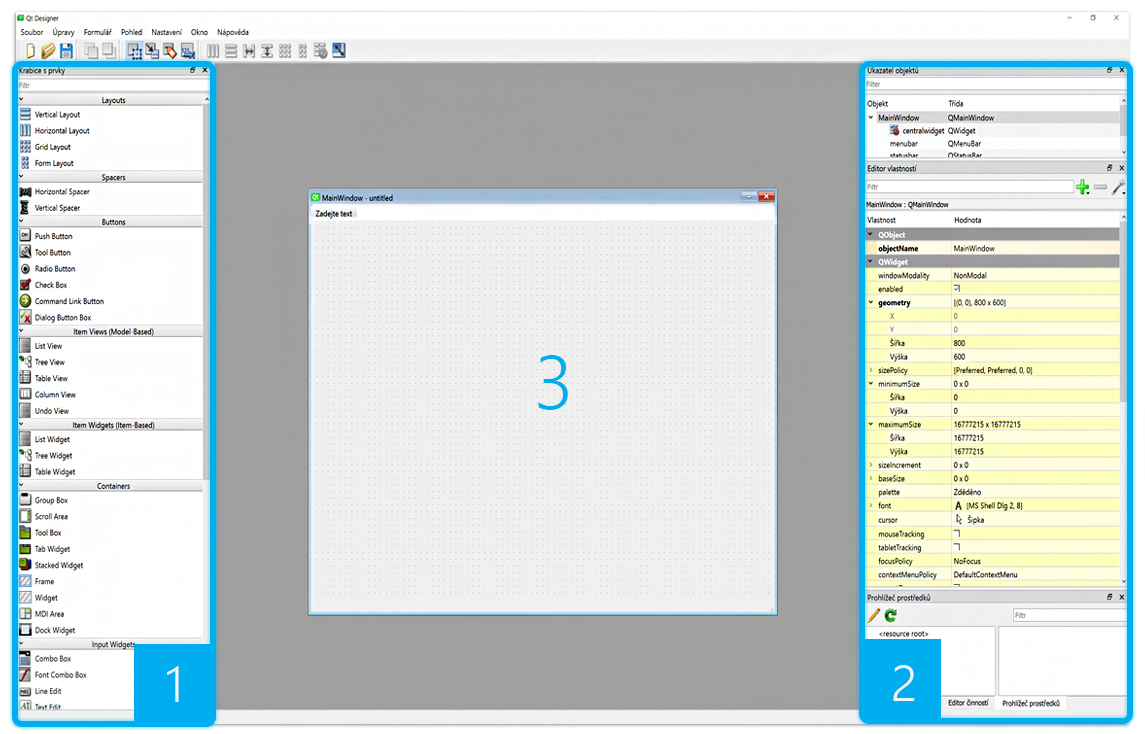
\includegraphics[width=1\textwidth]{bbpm/qt_designer}
        \caption{Prostředí \textit{Qt Designeru}}
        \label{fig:qt_designer}
    \end{center}
\end{figure}

\clearpage

Pro potřeby aplikace byly vytvořena dvě okna -- hlavní okno a okno nastavení.
Hlavní okno (viz Obr.~\ref{fig:app_main_window}) se skládá z postranního
vysouvacího menu~(\ref{fig:app_main_window}-\textbf{1}), které se nachází na
levé straně okna a panelu~(\ref{fig:app_main_window}-\textbf{2}), ve kterém se
zobrazuje karta podle zvolené položky v menu. Vysouvací menu obsahuje čtyři
tlačítka, přičemž první tlačítko, které se nachází v levém horním rohu hlavního
okna, iniciuje vysunutí a zasunutí menu. Jednotlivé funkce ostatních tlačítek
jsou:
\begin{itemize}[noitemsep]
    \item \textbf{Dashboard} -- zobrazení hlavní karty vizualizující výstup,
    \item \textbf{Record} -- zapnutí nahrávání EKG záznamu,
    \item \textbf{Settings} -- vyvolání dialogového okna s nastavením.
\end{itemize}
Postranní menu je modulární, což umožňuje snadné přidání nových položek a k nim
přidružených karet v pravém panelu. Modularita některých funkcí aplikace tak
zajišťuje snadnou rozšiřitelnost v budoucnu.

\begin{figure}[h]
    \begin{center}
        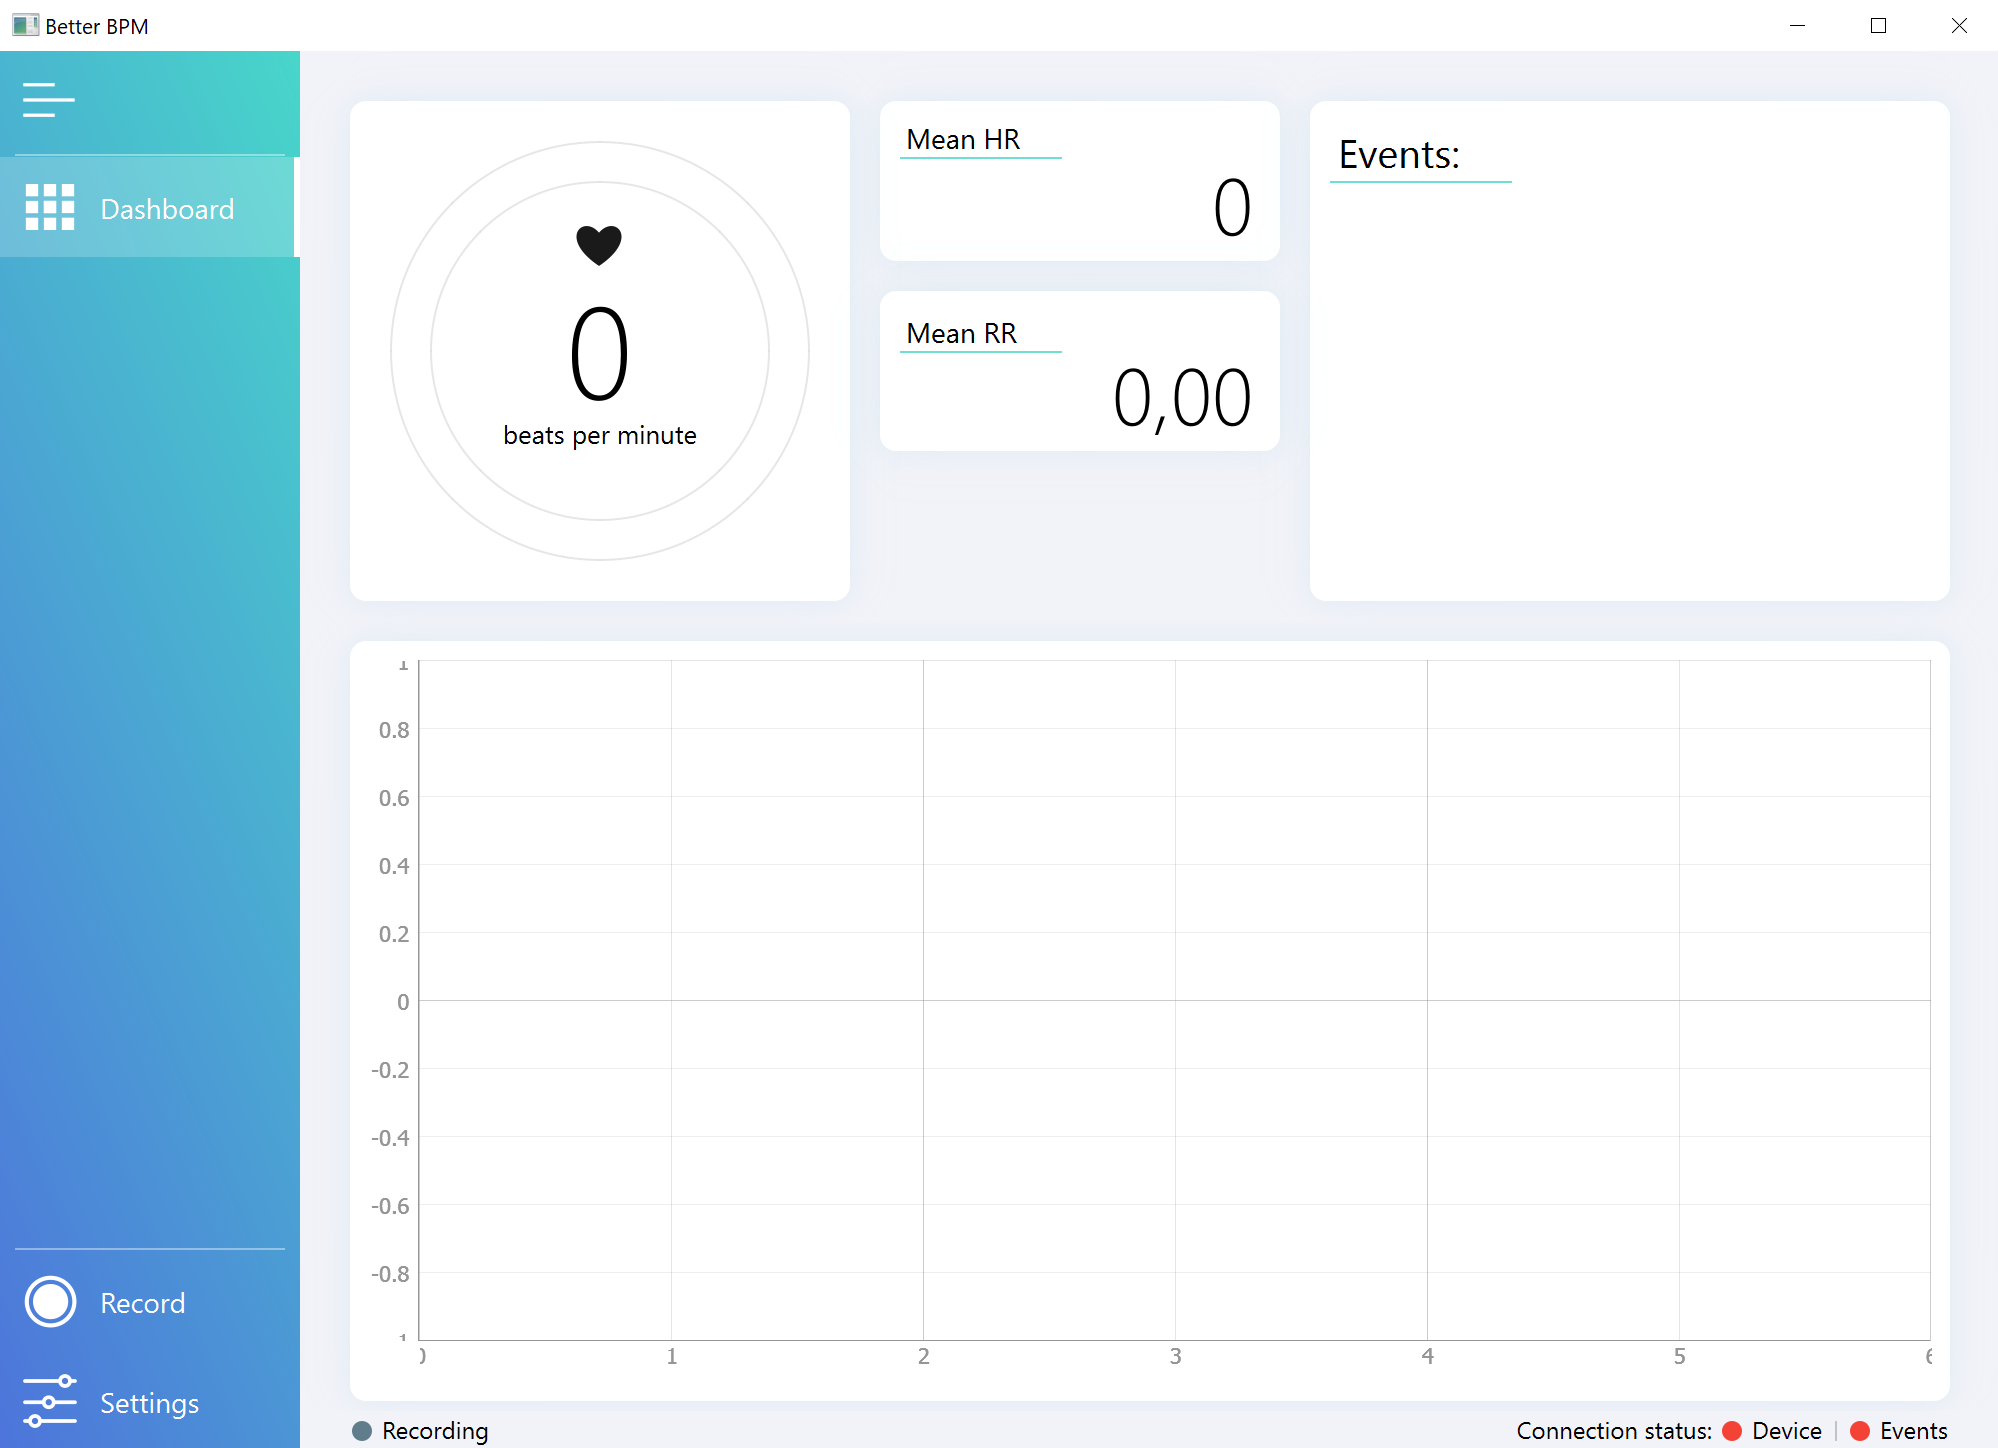
\includegraphics[width=1\textwidth]{bbpm/main_window}
        \caption{Struktura hlavního okna aplikace}
        \label{fig:app_main_window}
    \end{center}
\end{figure}

Karta \textbf{Dashboard} se skládá ze dvou segmentů. Dolní segment karty je
tvořen grafem pro zobrazení EKG křivky~(\ref{fig:app_main_window}-\textbf{4}),
který je detailněji popsán v sekci~\ref{section:visual}. Horní
segment~(\ref{fig:app_main_window}-\textbf{3}) obsahuje čtyři informační
subpanely. První tři zobrazují aktuální srdeční frekvenci, průměrnou srdeční
frekvenci a průměrnou délku R-R intervalů za posledních 6 sekund. První subpanel
zobrazující srdeční frekvenci, zároveň barevně indikuje, zda je její hodnota ve
fyziologickém rozmezí (zelená) nebo je zvýšená, snížená (oranžová) či abnormální
(červená). Rozmezí hodnot bylo zvoleno na základě stanoviska Americké
kardiologické asociace (AHA).

\begin{table}[h]
    \captionsetup{font=small,skip=0.5pt}
    \label{tab:aha_table}
    \catcode`\-=12
    \begin{center}
        \caption{Stanovené hodnoty srdeční frekvence podle AHA}
        \vspace{1ex}
        \setlength{\tabcolsep}{20pt}
        \renewcommand{\arraystretch}{1.3}
        \begin{tabular}{lcc}
            \noalign{\hrule height 2pt}
            \textbf{Srdeční rytmus} &  & \textbf{hodnota (bpm)} \\ \hline
            Bradykardie             &  & < 60                   \\
            Normální                &  & 60--100                \\
            Tachykardie             &  & > 100                  \\ \noalign{\hrule height 2pt}
        \end{tabular}
    \end{center}
\end{table}

Poslední informační subpanel (Events) má uplatnění během měření a hodnocení osob
ve VR v rámci výzkumu \textit{Virtuální město –- herní systém pro kognitivní
    trénink ve virtuálním prostředí}, zmíněného v úvodu
kapitoly~\ref{section:online_processing}. V této práci nemá využití, a proto
není dále blíže popsán.

Okno nastavení obsahuje čtyři záložky (viz Obr. \ref{fig:settings_cards}):
\begin{itemize}
    \item \textbf{General} (Obr.~\ref{fig:settings_general}) -- slouží pro
          nastavení připojovacích údajů k měřícímu zařízení. Tlačítkem \textbf{Test
              connection} lze zkontrolovat připojení.
    \item \textbf{Graph} (Obr.~\ref{fig:settings_graph}) -- slouží k nastavení
          grafu, konkrétně jeho vykreslovacích vlastností. Lze zde nastavit barva a
          tloušťka křivky nebo schovat osy a grid.
    \item \textbf{Recording} (Obr.~\ref{fig:settings_recording}) -- slouží k
          nastavení ID a jména měřené osoby, které se po nahrávání uloží
          společně s naměřenými daty.
    \item \textbf{Info} -- obsahuje informace o verzi aplikace a copyright.
\end{itemize}

\begin{figure}[h]
    \centering
    \begin{subfigure}[t]{0.3\textwidth}
        \centering
        \textcolor{cyan}{\fboxrule=0.5pt\fboxsep=0pt\fbox{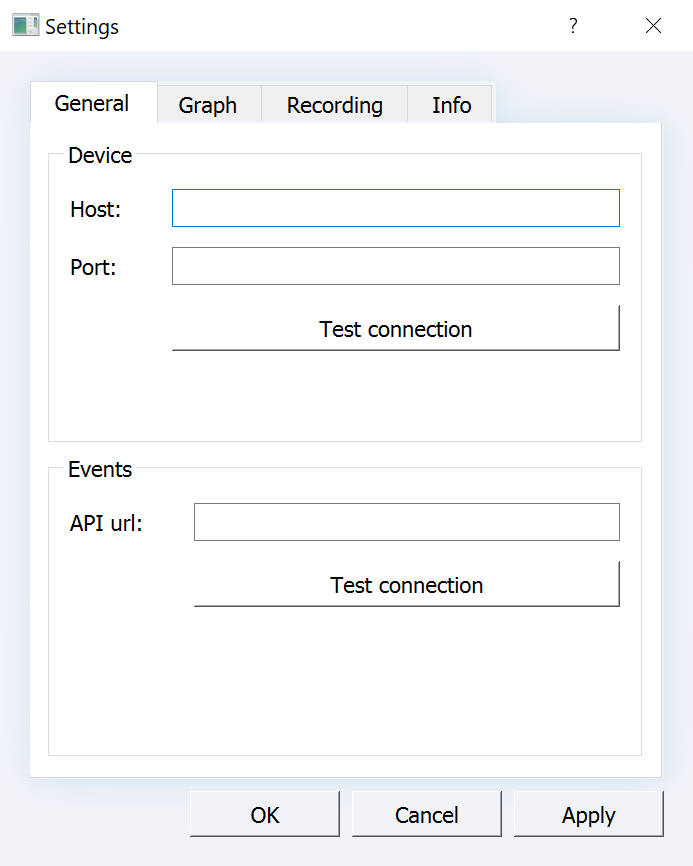
\includegraphics[width=1.05\linewidth]{bbpm/settings_general}}}
        \caption{záložka General}
        \label{fig:settings_general}
    \end{subfigure}
    \hspace{5pt}
    \begin{subfigure}[t]{0.3\textwidth}
        \centering
        \textcolor{cyan}{\fboxrule=0.5pt\fboxsep=0pt\fbox{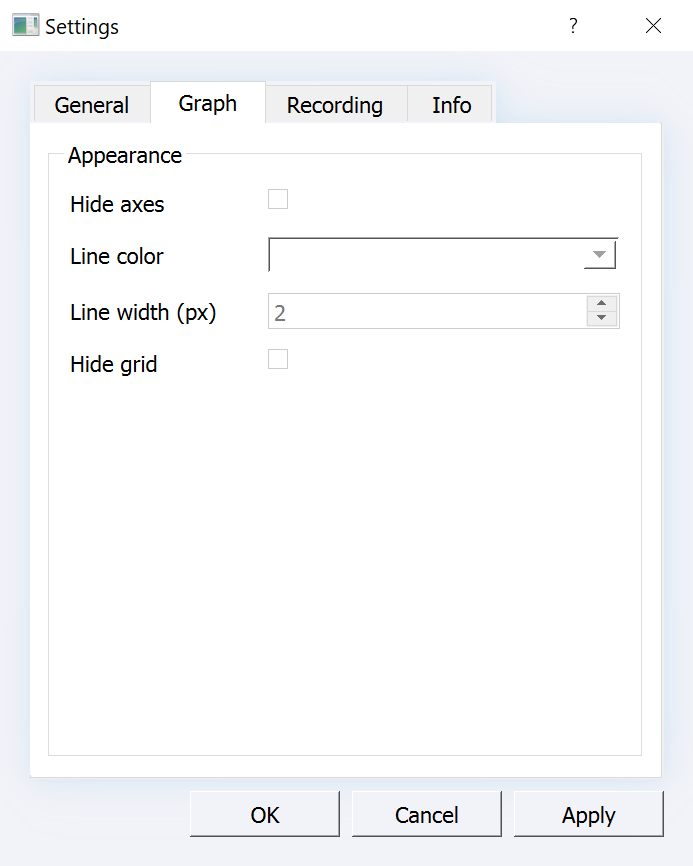
\includegraphics[width=1.05\linewidth]{bbpm/settings_graph}}}
        \caption{záložka Graph}
        \label{fig:settings_graph}
    \end{subfigure}
    \hspace{5pt}
    \begin{subfigure}[t]{0.3\textwidth}
        \centering
        \textcolor{cyan}{\fboxrule=0.5pt\fboxsep=0pt\fbox{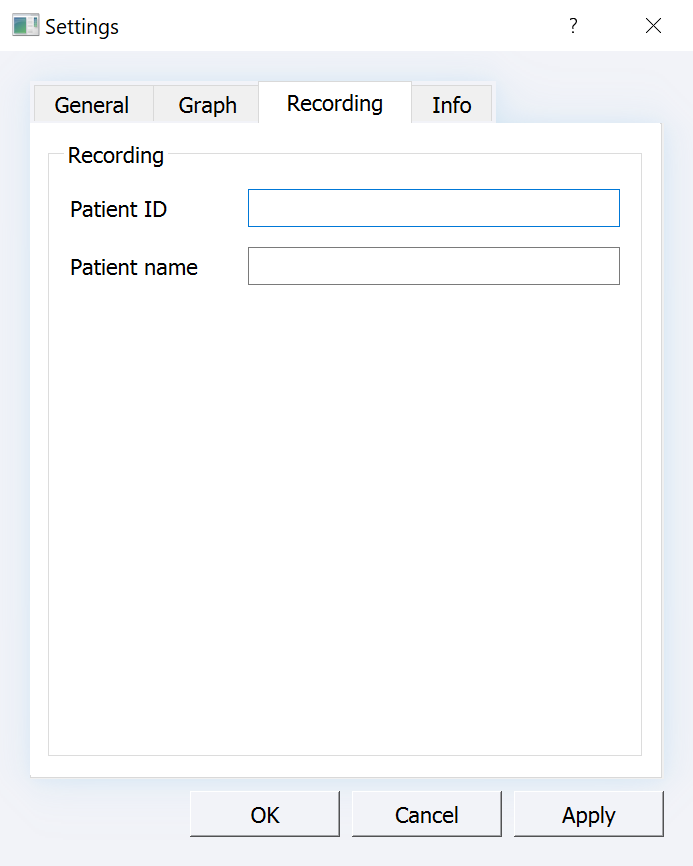
\includegraphics[width=1.05\linewidth]{bbpm/settings_recording}}}
        \caption{záložka Recording}
        \label{fig:settings_recording}
    \end{subfigure}
    \caption{Jednotlivé záložky v okně Nastavení}
    \label{fig:settings_cards}
\end{figure}

\subsubsection{Zpracování dat}
\label{section:online_data_process}
Pro zpracování dat jsou využívané funkce prostředí Python a knihovny
\textit{SciPy}~\cite{SciPy2020}. Před zpracováním EKG signálu jsou přijatá data
nejdříve upravena. Aplikace přijímá z měřícího zařízení v každý jeden okamžik
blok synchronizovaných dat v podobě dvou vektorů o velikosti 2048 hodnot. Jeden
vektor obsahuje hodnoty EKG signálů a druhý časové značky. 

\begin{figure}[h]
    \begin{center}
        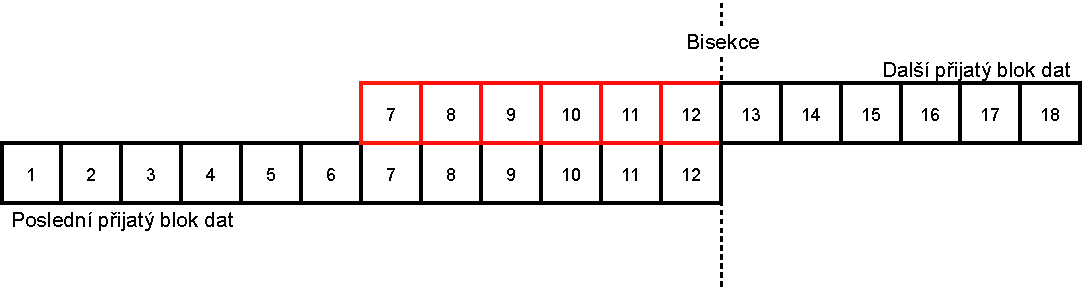
\includegraphics[width=0.9\textwidth]{figures/bisection}
        \caption{Bisekce překrývajících se dat}
        \label{fig:bisection}
    \end{center}
\end{figure}

Jednotlivě přijaté bloky na sebe nenavazují, ale překrývají se (viz Obr.~\ref{fig:bisection}). 
Kontinuita dat je zajištěna použitím algoritmu bisekce, realizovaného funkcí
\texttt{bisect(a,x)}~\cite{bisectRight}, který najde index prvního navazujícího
prvku v závislosti na poslední hodnotě časového vektoru minulého bloku dat.
Překrývající data před tímto indexem jsou odstraněna a podle takto upraveného
časového vektoru je následně upraven i vektor s EKG daty.

Upravené bloky EKG dat jsou předzpracovány filtrem
Savitzky–Golay~(SGF)~\cite{Schafer2011} použitím funkce
\texttt{savgol{\_}filter(x,win{\_}length,order)}~\cite{scipySavgol}. 
SGF je digitální filtr s konečnou impulzní odezvou (FIR), který se
nejčastěji používá k vyhlazení signálu a potlačení jeho vysokofrekvenční složky.
Princip filtru SGF vychází z proložení hodnot v plovoucím okně polynomem
určitého řádu využitím metody nejmenších čtverců. Výsledná hodnota signálu v
daném bodě je vypočtena jako~\cite{wikiSGF}:
\begin{equation}
    y_j = \sum_{i=\frac{1-M}{2}}^{\frac{M-1}{2}} c_j y_{j+i}, \quad \frac{M-1}{2} \leq j \leq N - \frac{M-1}{2}
\end{equation}
kde $c_j$ jsou vypočítané koeficienty polynomiální regrese, $M$ je délka
plovoucího okna a $N$ délka signálu. V aplikaci byla zvolena délka okna 151
vzorků a polynom 3. řádu. Příklad SGF filtrace se zvolenými parametry lze vidět
na Obr.~\ref{fig:sgf_filter}.

Po filtraci jsou data přidána do cyklické fronty~\cite{circlebuffer}, kde
probíhá nepřetržitá detekce komponentů, konkrétně R vln. K detekci je použita
funkce \texttt{find{\_}peaks(x,h,d)}~\cite{scipyFindpeaks}. Funkcí probíhá
hledání lokálních maxim signálu v závislosti na zadané prahové amplitudě a
minimální vzdáleností mezi sousedními R vlnami. Prahová hodnota amplitudy byla
zvolena 0,2~\si\mV~a minimální vzdálenost 0,4~\si\s~(200 vzorků).

\begin{figure}[h]
    \begin{center}
        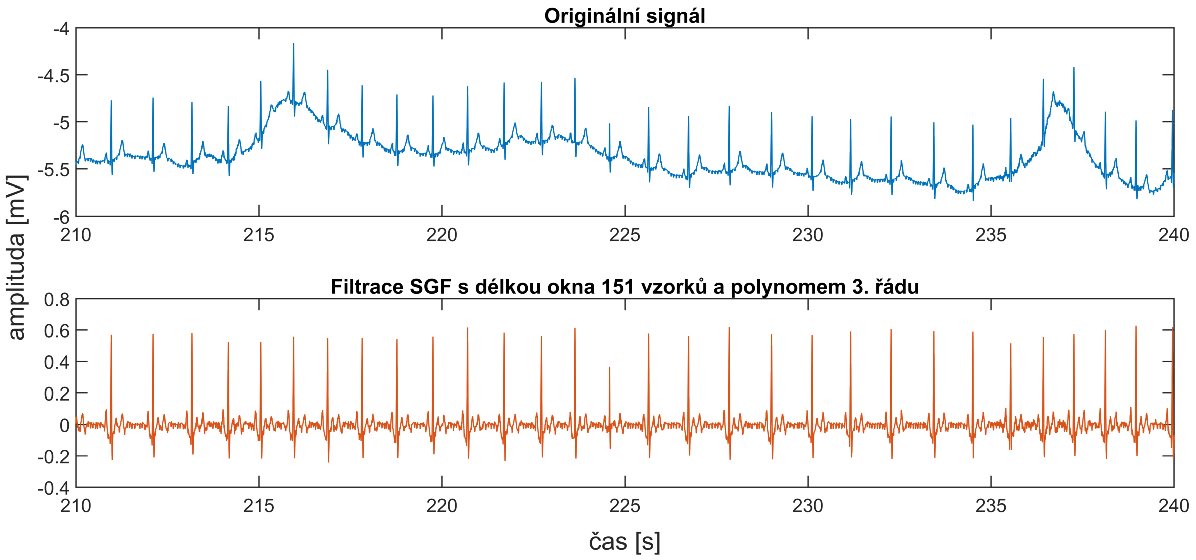
\includegraphics[width=1\textwidth]{figures/sgf_filter}
        \caption{Savitzky–Golay filtrace}
        \label{fig:sgf_filter}
    \end{center}
\end{figure}

Zpracování komponentů (R vln) se odvíjí od zobrazených parametrů na hlavním
panelu aplikace (viz Obr. \ref{fig:app_main_window}). Detekované R vlny slouží k 
výpočtu srdeční frekvence. Diferencí časových hodnot R vln jsou získány R-R intervaly. 
Aktuální srdeční frekvence je poté vypočtena použitím posledního R-R intervalu následovně:
\begin{equation}
    \label{eq:calc_hr}
    HR = \frac{60}{RR}
\end{equation}
kde $HR$ je hodnota srdeční frekvence a $RR$ aktuálně vypočtená srdeční
perioda. Na panelu je z vypočítané hodnoty zobrazena celá část čísla. Dalším
parametrem je průměrná hodnota srdeční frekvence, která se počítá podle
vztahu~\ref{eq:calc_hr} výše. Namísto $RR$ je ale dosazena průměrná hodnota
všech R-R intervalů za posledních 6 sekund, která je posledním počítaným
parametrem podle:
\begin{equation}
    \overline{RR} = \frac{1}{N} \sum_{i=1}^N RR_i
\end{equation}
kde $\overline{RR}$ je vypočítaný průměr R-R intervalů a $N$ je počet R-R
intervalů. Hodnoty se následně zobrazují na panelu v horním segmentu aplikace.

\subsubsection{Vizualizace EKG}
\label{section:visual}
Pro vykreslování dat je použita knihovna \textit{PyQtGraph} \cite{PyQtGraph},
která je plně kompatibilní s frameworkem \textit{PySide2} (viz
sekce~\ref{section:pyside}). Hlavním komponentem této knihovny je graf, kterému
lze funkcí \texttt{setData(x,y)}~\cite{curveItem} předat hodnoty pro osu X a Y.
Po předání jsou hodnoty vykresleny a graf je aktualizován. Předávání hodnot se 
provádí cyklicky, a tak dochází
\begin{figure}[H]
    \begin{center}
        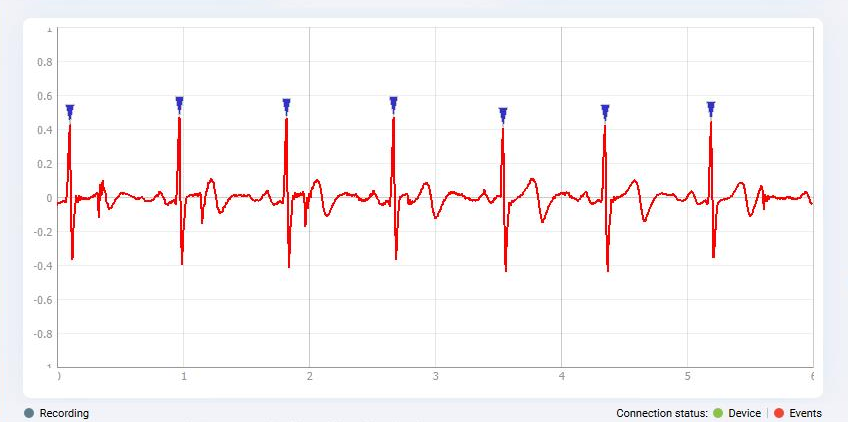
\includegraphics[width=0.75\textwidth]{bbpm/r_detection}
        \caption{Vizualizace EKG křivky s detekcí R vln na hlavním panelu
        aplikace \textit{BBPM}}
        \label{fig:app_ecg_visual}
    \end{center}
\end{figure}
\noindent k neustálému vykreslování nových EKG dat. Zároveň jsou využity hodnoty
detekovaných R vln pro vykreslování markerů v podobě modrých šipek, které tyto
vlny označují. Vizualizace dat na hlavním panelu je vidět na
Obr.~\ref{fig:app_ecg_visual}.

\subsection{Statistické metody}
\label{section:statistical_methods}
Pro zpracování výsledků byly v práci použity statistické testy realizované
funkcemi v prostředí programu \textit{MathWorks MATLAB 2021a}~\cite{MATLAB},
které prověřují platnost nulové hypotézy $H_0$. Nulová hypotéza představuje ve
většině případů tvrzení, že rozdíl mezi testovanými daty není statisticky
významný. Proti $H_0$ se zavadí alternativní hypotéza $H_A$, která nulovou
hypotézu vyvrací. K určení platnosti mezi testovanou nebo alternativní hypotézou
slouží statistické testování, které probíhá následovně:
\begin{itemize}
    \item Definice nulové hypotézy $H_0$ s předpokladem, že platí.
    \item Stanovení náhodného pokusu, kterým bude ověřena hypotéza a náhodné
          veličiny, která bude výsledkem pokusu.
    \item Zvolení hladiny významnosti \textalpha, která vyjadřuje
          pravděpodobnost neoprávněného zamítnutí nulové hypotézy $H_0$, i když platí.
          V bakalářské práci je zvolena hladina významnosti \textalpha~=~0,05 (5~\%).
    \item Zamítnutí nulové hypotézy $H_0$ v případě, že hodnota náhodné veličiny
          spadá do kritického oboru, jelikož nastal jev, který by byl velmi
          nepravděpodobný za platnosti hypotézy $H_0$.
    \item Vyhodnocení statistického testu na základě rozhodnutí o platnosti
          nulové hypotézy $H_0$: přijetí hypotézy $H_0$ (zamítnutí alternativní
          hypotézy $H_A$) nebo zamítnutí hypotézy $H_0$ (přijetí alternativní
          hypotézy $H_A$).
\end{itemize}

Pro testování normality náhodné veličiny byl zvolen Shapirův-Wilkův
test~\cite{wikiSHAPIROWILK} na základě porovnání síly testů pro malé vzorky
podle~\cite{Razali2011}. Nulová hypotéza testu $H_0$ tvrdí, že testovaný vzorek
dat pochází z populace s normálním rozdělením. Test byl proveden použitím funkce
\texttt{swtest(x)}~\cite{matlabSWTEST}.

\subsubsection{Parametrické testy}
\label{section:parametric_tests}
Parametrické varianty testů mohou být uplatněny pouze při splnění podmínky
normality dat. V práci byl použit párový t-test~\cite{Henry2005}, který testuje
rozdíl středních hodnot mezi dvojicí veličin dvourozměrného náhodného výběru.
Test byl realizován funkcí \texttt{ttest(x)}~\cite{matlabTTEST}.